%% Copyright 2007-2025 Elsevier Ltd
%% 
%% This file is part of the 'Elsarticle Bundle'.
%% ---------------------------------------------
%% 
%% It may be distributed under the conditions of the LaTeX Project Public
%% License, either version 1.3 of this license or (at your option) any
%% later version.  The latest version of this license is in
%%    http://www.latex-project.org/lppl.txt
%% and version 1.3 or later is part of all distributions of LaTeX
%% version 1999/12/01 or later.
%% 
%% The list of all files belonging to the 'Elsarticle Bundle' is
%% given in the file `manifest.txt'.
%% 
%% Template article for Elsevier's document class `elsarticle'
%% with harvard style bibliographic references

\documentclass[preprint,12pt]{elsarticle}

%% Use the option review to obtain double line spacing
%% \documentclass[authoryear,preprint,review,12pt]{elsarticle}

%% Use the options 1p,twocolumn; 3p; 3p,twocolumn; 5p; or 5p,twocolumn
%% for a journal layout:
%% \documentclass[final,1p,times,authoryear]{elsarticle}
%% \documentclass[final,1p,times,twocolumn,authoryear]{elsarticle}
%% \documentclass[final,3p,times,authoryear]{elsarticle}
%% \documentclass[final,3p,times,twocolumn,authoryear]{elsarticle}
%% \documentclass[final,5p,times,authoryear]{elsarticle}
%% \documentclass[final,5p,times,twocolumn,authoryear]{elsarticle}

%% For including figures, graphicx.sty has been loaded in
%% elsarticle.cls. If you prefer to use the old commands
%% please give \usepackage{epsfig}

%% The amssymb package provides various useful mathematical symbols
\usepackage{amssymb}
%% The amsmath package provides various useful equation environments.
\usepackage{amsmath}
\usepackage{booktabs}  % optional, for better-looking tables
\usepackage{threeparttable}
\usepackage{xcolor}
\usepackage{subcaption}
\usepackage[utf8]{inputenc}
\usepackage{multirow}
\usepackage{amssymb}
\usepackage{tabularx} % For adjustable width columns
\usepackage{enumitem} % For customizing lists within the table
%% The amsthm package provides extended theorem environments
%% \usepackage{amsthm}
\usepackage{hyperref}
\hypersetup{
    colorlinks=true,
    linkcolor=blue,
    filecolor=magenta,      
    urlcolor=cyan,
    }
\usepackage{graphicx}
\usepackage{makecell}
\usepackage{soul}

\usepackage{enumitem} % Allows for tighter bullet lists

% Custom column type to center the first column while keeping it fixed width
\newcolumntype{C}{>{\centering\arraybackslash}p{2.5cm}}

% Custom command to make itemized lists look good inside tables
\newlist{tablelist}{itemize}{1}
\setlist[tablelist]{
    label={},
    nosep,                 % Removes vertical space between items
    leftmargin=*,          % Aligns bullets to the left
    before=\vspace{0pt},   % Important: aligns the top of the list with the row
    after=\vspace{-\baselineskip} % Prevents extra space at the bottom
}

%% The lineno packages adds line numbers. Start line numbering with
%% \begin{linenumbers}, end it with \end{linenumbers}. Or switch it on
%% for the whole article with \linenumbers.
%% \usepackage{lineno}

\journal{Nuclear Physics B}

\begin{document}

\begin{frontmatter}

%% Title, authors and addresses

%% use the tnoteref command within \title for footnotes;
%% use the tnotetext command for theassociated footnote;
%% use the fnref command within \author or \affiliation for footnotes;
%% use the fntext command for theassociated footnote;
%% use the corref command within \author for corresponding author footnotes;
%% use the cortext command for theassociated footnote;
%% use the ead command for the email address,
%% and the form \ead[url] for the home page:
%% \title{Title\tnoteref{label1}}
%% \tnotetext[label1]{}
%% \author{Name\corref{cor1}\fnref{label2}}
%% \ead{email address}
%% \ead[url]{home page}
%% \fntext[label2]{}
%% \cortext[cor1]{}
%% \affiliation{organization={},
%%            addressline={}, 
%%            city={},
%%            postcode={}, 
%%            state={},
%%            country={}}
%% \fntext[label3]{}

\title{Safety First --- A Systematic Literature Review on the Impact of AI on High-Stakes Decision-Making} %% Article title

%% use optional labels to link authors explicitly to addresses:
%% \author[label1,label2]{}
%% \affiliation[label1]{organization={},
%%             addressline={},
%%             city={},
%%             postcode={},
%%             state={},
%%             country={}}
%%
%% \affiliation[label2]{organization={},
%%             addressline={},
%%             city={},
%%             postcode={},
%%             state={},
%%             country={}}

\author{Nataly R. Panczyk} %% Author name
\author{Riley J. Fisher}
\author{Majdi I. Radaideh}

%% Author affiliation
\affiliation{organization={Department of Nuclear Engineering and Radiological Sciences, University of Michigan Ann Arbor},%Department and Organization
            addressline={2355 Bonisteel Blvd.}, 
            city={Ann Arbor},
            postcode={48105}, 
            state={Michigan},
            country={USA}}

%% Abstract
\begin{abstract}
%% Text of abstract
Abstract text.
\end{abstract}

%%Graphical abstract
% \begin{graphicalabstract}
%
\includegraphics{grabs}
% \end{graphicalabstract}

%%Research highlights
% \begin{highlights}
% \item Research highlight 1
% \item Research highlight 2
% \end{highlights}

%% Keywords
\begin{keyword}
%% keywords here, in the form: keyword \sep keyword
AI-Informed Decision-Making \sep Sensitive Industries \sep Systematic Literature Review

\end{keyword}

\end{frontmatter}

\fbox{
\parbox{0.8\textwidth}{
    \textbf{REVIEW KEY:} \\
    \textcolor{red}{General questions and things to double-check.} \\
    \hl{Specific phrases that need review.} \\
    \textcolor{cyan}{Things Riley needs to do or check.} \\
    \textcolor{green}{Specific notes for Majdi.} \\
    \st{Stuff you'd like Nataly to cut.} \\
    \textbf{*DON'T USE OVERLEAF COMMENTS!} \\
    This will almost certainly break the Github-Overleaf sync. \\
}}

\section{Introduction}

The goal of this review is to explore safety-critical applications that have attempted or considered introducing artificial intelligence (AI) to their domains for decision-making purposes. We specifically exclude the use of AI for exploratory purposes to limit our scope to scenarios in which \textit{human lives may be at risk}. While applications for the modern surge of AI-based technologies abound, we sought to identify the subset requiring the strictest scrutiny via its potential to cause the most harm. Our approach to identifying this subset was, as the title suggests, systematic. We cast a wide net in our search, then filter with a series of criteria, which we outline in Section \ref{sec:methods}. After distilling our initial pool of 1,135 papers into a final subset of 72 reports, we have identified critical features of both AI technology and implementation practices that span domain boundaries. Throughout this review, we explore patterns across these industries that demonstrate common failure modes, barriers to successful implementation, and limiting factors to status quo improvement with these technologies. The papers in this review range from software design and technical evaluations to legal reviews and qualitative studies with users and experts from the various domains. As such, while this paper was written by engineers, we anticipate its findings to interest regulators, practitioners, and participants of a variety of industries, alike. Table \ref{tab:industry_categorization} shows the industries considered in this review and the varying features of safety-critical decision-making they cover. \textcolor{cyan}{@Riley, add stuff here!}

\begin{table}
    \centering
    \begin{tabular}{lrrrr}
        \toprule
        Industry & Accident Freq. & Affected Pop. & Interfacing User & Time to Decide \\
        \midrule
        Medical & High & Low & Highly Skilled & Minutes-Days \\
        & & & or Public \\
        Autonomous & Medium & Medium & Public & Seconds \\
        Vehicles & & & & \\
        Aviation & Low & Medium-High & Highly Skilled & Seconds-Minutes \\
        Nuclear & Very Low & Very High & Highly Skilled & Minutes-Days\\
        \bottomrule
    \end{tabular}
    \caption{General spread of accident frequency, the size of the affected population when an accident does occur, the possible interfacing users, and decision timeline for the industries considered in this analysis. \textcolor{red}{Need help formatting this!!!}}
    \label{tab:industry_categorization}
\end{table}
\section{Methods}
\label{sec:methods}

\textcolor{red}{Make sure this is true!} This analysis follows the Preferred Reporting Items for Systematic reviews and Meta-Analyses (PRISMA) methodology and therefore collects documents in a systematic and automated way. To do so, we start by defining the research questions this review seeks to answer. These include, the titular: \textit{What is the impact of AI on high-stakes decision-making?} As well as: \textit{How are safety outcomes perturbed by AI-based decision-making in sensitive industries?} And \textit{What are the safety risks of using AI to make decisions in sensitive industries?} While there are benefits and harms to using AI-based technologies, that comparison alone is far too high-level to inspire targeted change within the AI technologies themselves. The nature of the questions guiding this review probe at what unique features and outcomes set AI-based decision-making mechanisms apart from traditional methods. Understanding these phenomena in detail would allow useful insight for both governmental agencies and engineers to mitigate evident shortcomings of this high-impact technology. \textcolor{cyan}{@Riley, if you don't like the location of the table discussion, optionally move it here.}

\subsection{Query Term Compilation}
After determining our research questions, we define a set of key terms using the Population, Intervention, Comparison, Outcome (PICO) methodology, and use the Cartesian product of these terms (one from each category) to determine relevant search queries. We use APIs for each of two databases, Scopus and Web of Science, to make these queries via a Python workflow, storing all resultant papers. Then, we remove duplicates based on digital object identifier (DOI), and merge the results of both database searches into a combined bibliography. Figure \ref{fig:workflow} shows visual representation of this workflow. 

\begin{figure}
    \centering
    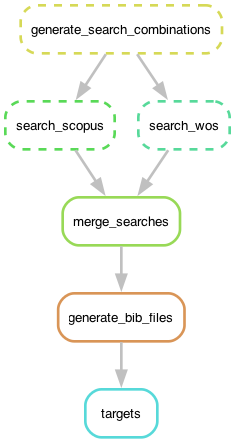
\includegraphics[width=0.5\linewidth]{figs/dag.png}
    \caption{Directed acyclic graph showing automatic search workflow.}
    \label{fig:workflow}
\end{figure}

Critical to actually making these queries is defining the lists of keywords that comprise them. We start by defining our population terms.  


We can organize the population terms we decided to include in this search in five major groups: nuclear and radiation, aviation, autonomous driving, energy and industrial processes, and medical technology and pharmaceuticals. These groups were selected for their highly sensitive nature, their propensity to use AI, and their regulatory authorities. This includes oversight by the U.S. Nuclear Regulatory Commission (NRC), the Federal Aviation Administration (FAA), the National Highway Traffic Safety Administration (NHTSA), the Occupational Health and Safety Administration (OSHA), and the Food and Drug Administration (FDA). There are a vast number of industries that might be considered ``sensitive'' and are federally regulated in the United States, however, due to time and space limitations, we prioritize those listed above in our analysis. While we included three query terms that did explicitly include some of these regulatory bodies (see Table \ref{tab:search_terms}), we found our more general terms sufficient to cover international bodies. Specifically, our goal was to avoid cases that consider risks \textit{not imminently} related to human health and safety (financial risks, environmental risks); we will discuss this further when we consider our exclusion criteria. The population search terms we include in our querying are shown in Table \ref{tab:search_terms}. 

After determining our population terms, we then must consider our intervention terms. We determined this group by compiling a list of AI-related terms that would likely appear in any AI-based decision-making model. This includes words and phrases like ``machine learning,'' ``neural networks,'' and ``language models.'' In our full query, which we describe later in this section, we use the search operator \verb|W/5| and \verb|NEAR/5| for Scopus and Web of Science, respectively, to pair each intervention term in Table \ref{tab:search_terms} with the wildcard term ``decision*''. In lieu of a mere \verb|AND| operator, these operators require the word ``decision'' and its derivatives to be within five words of the AI-intervention term. The objective of this pairing is to return articles that use AI to either make or inform some kind of decision. The criticality and sensitivity of that decision will be evaluated during later screening. The intervention search terms we include in our querying are shown in Table \ref{tab:search_terms}. 

Finally, we consider our outcome terms. Our research question focuses on the impact of AI-based decision-making on safety outcomes in sensitive industries. Thus, our outcome terms focus on safety, specifically, on risks to human health. We include general terms like ``incident,'' ``accident,'' and ``near miss,''  as well as more industry-specific terms, like ``misdiagnos*'' and ``operating experience.'' To ensure we capture any failures that led to official infractions, we included several regulation-specific terms, too, like ``FDA recall*'' and ``OSHA citation.'' A complete list of outcome terms used in our querying are shown in Table \ref{tab:search_terms}. 


\begin{table}[ht]
\centering
\caption{Search terms used to produce Cartesian-product-based queries}
\label{tab:search_terms}
\renewcommand{\arraystretch}{1.25}
\begin{tabular}{p{0.3\textwidth} p{0.29\textwidth} p{0.32\textwidth}}
\hline
\textbf{Population Terms} & \textbf{Intervention Terms} & \textbf{Outcome Terms} \\
\hline
nuclear & ``artificial intelligence'' & incident* \\
radiation & AI & ``close call*'' \\
aerospace & ``machine learning'' & accident* \\
aviation & ML & ``near miss*'' \\
aircraft & ``neural network*'' & injur* \\
airport & ``language model*'' & failure* \\
``autonomous driving'' & computer vision & ``adverse event*'' \\
``autonomous vehicle*'' & automated & malfunction \\
self-driving & ``deep learning'' & fatalit* \\
automotive* & & misdiagnos* \\
energy & & harm \\
``power grid*'' & & ``operating experience*'' \\
``electric grid*'' & & ``OSHA citation*'' \\
chemical & & ``FDA recall*'' \\
petroleum & & ``NHTSA investigation*'' \\
``medical device*'' & & violation* \\
``medical equipment'' & & ``enforcement action*'' \\
``diagnostic device*'' & & \\
``imaging device*'' & & \\
``surgical robot*'' & & \\
``implantable device*'' & & \\
drug* & & \\
``patient safety'' & & \\
pharmaceutical* & & \\
radiotherapy & & \\
``clinical trial*'' & & \\
\hline
\end{tabular}
\begin{tablenotes}
\small
\item Note: Asterisks (*) indicate truncation wildcards.
\end{tablenotes}
\end{table}

\subsection{Search Process}
The goal of our search process was to search two databases, Scopus and Web of Science, for all articles containing our four primary search terms in their title, abstract, or keywords. We imposed two additional requirements, that the papers be published after and not including 2014 and that the papers either be journal articles or conference papers from the top five AI conferences as listed by Google Scholar Metrics \cite{google_scholar_metrics}. This conference paper subset includes \textit{Neural Information Processing Systems}(NEURIPS), the \textit{International Conference on Learning Representations} (ICLR), the \textit{International Conference on Machine Learning} (ICML), the \textit{AAAI Conference of Artificial Intelligence} (AAAI), and the \textit{International Joint Conference on Artificial Intelligence} (IJCAI). We created this subset using the combination of both a paper type of \texttt{conference proceedings} and that conference proceeding containing one of the five acronyms listed above. In the case that this search catches an additional conference, that paper will be excluded during the abstract screening phase. 

We combined our search terms into the following query search:
\begin{quote}
\texttt{TITLE-ABS-KEY ( \{population term\} ) AND TITLE-ABS-KEY ( \{intervention AI term\} within five words of \{decision*\}) AND TITLE-ABS-KEY ( \{outcome term\} ) AND PUBLICATION YEAR AFTER 2014 AND (DOCUMENT TYPE(article) OR (DOCUMENT TYPE(conference proceeding) AND \{conference subset\}))}
\end{quote}

Note: the query format above matches Scopus syntax most closely, but is intended for demonstrative purposes only. We show our exact query structure in the \textcolor{red}{code repository}. The final set of articles considered for this analysis was pulled from both Scopus and Web of Science on December 15, 2025.


As shown in Figure \ref{fig:workflow}, after searching the full set of queries in both Scopus and Web of Science, merging the search results into a single database and dropping duplicates based on DOI, we generated a singular bibliographic file in the \verb|.bib| structure. We then loaded the bibliographic information into Zotero. \hl{Zotero flagged two articles as retracted, Mohanta et al. and Ponraj et al.} \textcolor{red}{Not sure if we should call these out.} We removed these records in the pre-screening phase along with one manually identified duplicate record. This yielded a total of 630 records for screening. Figure \ref{fig:prisma_flow} shows the number of articles retained at each phase of the filtration process.

\begin{figure}[ht!]
  \centering
  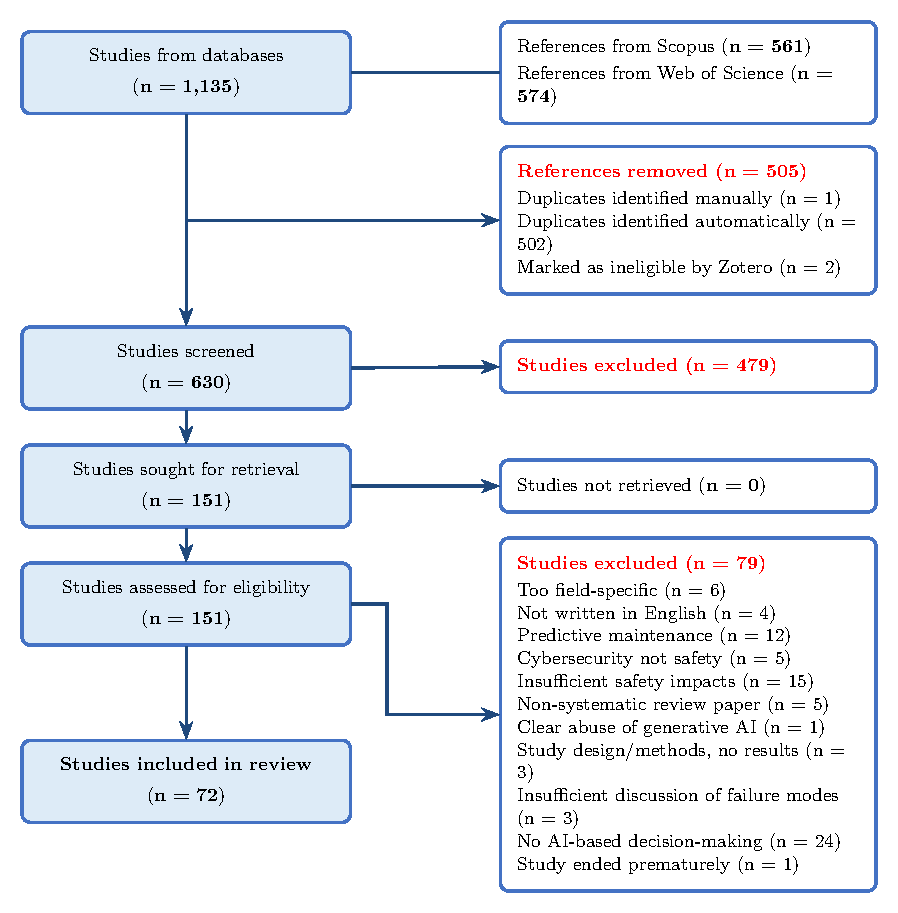
\includegraphics[width=\textwidth]{figs/prisma_flow.pdf} 
  \caption{PRISMA flow diagram.}
  \label{fig:prisma_flow}
\end{figure}

\subsection{Screening Process}
% Discuss inclusion and exclusion criteria
Following the PRISMA methodology, we perform the screening process in two phases-- title and abstract screening, and full-text review. During the abstract screening, we followed the inclusion/exclusion criteria shown in Table \ref{tab:inclusion_exclusion}, keeping questionable articles conservatively based on what we read in the titles and abstracts \textit{only}. The purpose of this phase is to quickly remove all articles that absolutely do not meet our criteria, while keeping any that may. During the abstract screening, this mainly involved removing articles with an emphasis on outcomes that were not threats to human health or safety. 

% Explain predictive maintenance here
\textcolor{cyan}{@Riley, please review this paragraph after our discussion!}
We excluded many articles during this phase because they fell under the category of ``predictive maintenance.'' While predictive maintenance undoubtedly has value in a variety of industries, the goal of these types of studies almost always focuses on reducing costs via an optimized (read: less frequent) maintenance schedule. By this logic, predictive maintenance has no impact on safety, at best. Note that when AI used to predict equipment failures, without reducing maintenance frequency, we do not consider this predictive maintenance and include these studies in our review. We assume that in all mechanical systems, there exists a conservative measure to ensure failures do not occur at a higher rate, which is to follow the most frequent maintenance schedule. Because the safety-oriented solution in maintenance scenarios has a clear way to avoid harms caused by AI, and is fundamentally motivated as a cost-saving technique, we excluded predictive maintenance papers in our study unless they simultaneously presented a safety-critical aspect. More generally, we excluded all papers that sought to strictly reduce system costs with AI or enhance their system security in a way that did not impact human health or safety. Our main filtration system asked: \textit{Does this system have the potential to directly harm human lives?} Additional details provided in Table \ref{tab:inclusion_exclusion} help provide more complete picture. 

We also created exclusion criteria to define ``AI.'' Because we sought to consider regulatory approaches to AI in this analysis, we drew the line at pure linear regression based models and IF/ELSE-type logic models, since these algorithms are already widely accepted and \hl{straightforward to regulate} \textcolor{red}{is this true?}. Finally, we excluded any reviews that were non-systematic, any articles that were retracted, any ethics-based papers without a clear application to the AI technology or use of AI technology in their target domain, and any papers not written in English. \hl{To assist with our screening process, we used Covidence, a website designed for systematic reviews.} \textcolor{red}{Do we need to include this?} We did not track case-by-case reasons for exclusion during the abstract screening phase. As shown in Figure \ref{fig:prisma_flow}, we excluded 479 articles in this phase, yielding 151 articles for the full-text review process.


\begin{table}[h]
\renewcommand{\arraystretch}{1.5} % Adds a bit of breathing room
\begin{tabularx}{\textwidth}{CXX}
\hline
\textbf{} & \centering \textbf{Inclusion} & \centering\arraybackslash \textbf{Exclusion} \\ \hline

% Row 2
\textbf{Population} & 
\begin{tablelist}
    \item Sensitive technology (e.g., nuclear, aviation)
    \item Medical studies, emphasizing equipment, devices, and drugs
    \item 
\end{tablelist} & 
\begin{tablelist}
    \item Finance
    \item Human resources (even if health related)
    \item Cybersecurity
\end{tablelist} \\ \hline

% Row 3
\textbf{Intervention} & 
\begin{tablelist}
    \item AI-informed decision-making (with any degree of autonomy)
    \item 
\end{tablelist} & 
\begin{tablelist}
    \item Simple flow chart or IF/ELSE logic
    \item Linear regression models
\end{tablelist} \\ \hline

% Row 4
\textbf{Comparison} & 
\begin{tablelist}
    \item Human evaluation
    \item Deterministic method
\end{tablelist} & 
\begin{tablelist}
    \item ML-ML comparison (with exceptions)
    \item 
\end{tablelist} \\ \hline

% Row 5
\textbf{Outcome} & 
\begin{tablelist}
    \item Incidents, accidents, and failures
    \item Threat to human health
    \item Regulatory compliance violations
\end{tablelist} & 
\begin{tablelist}
    \item Non-threat to human health risks
    \item Financial risks or economic losses
    \item Cyber or other security risks
    \item 
\end{tablelist} \\ \hline

% Row 6
\textbf{Other} & 
\begin{tablelist}
    \item Peer-reviewed journal articles
    \item Select conference papers
    \item 
\end{tablelist} & 
\begin{tablelist}
    \item Non-systematic review papers
    \item Retracted articles
    \item Ethics without application
    \item Not written in English
    \item Published before 2015
    \item 
\end{tablelist} \\ \hline

\end{tabularx}
\caption{Inclusion and exclusion criteria used for abstract screening phase.}
\label{tab:inclusion_exclusion}
\end{table}

\subsection{Full Text Screening}
After the title and abstract screening, we proceeded to the full text screening stage. This phase, as its name suggests, involves reading the full text of each paper and applying the same inclusion/exclusion criteria shown in Table \ref{tab:inclusion_exclusion}. The articles that made it past the abstract phase showed promise for meeting all of our inclusion criteria, but this must be confirmed after fully analyzing each text. During the full-text screening phase, we track the exclusion reason for each article. The number of articles and their specific exclusion criteria are shown in Figure \ref{fig:prisma_flow}. 

We did include some additional exclusion reasons during this phase to increase our specificity. One example was the note: ``too field-specific.'' This was only a handful of papers, but consisted of studies that failed to discuss the AI technology in sufficient detail or conversely, failed to discuss the AI application in specific detail. Similarly, we did not include methods-only papers. One paper we reviewed showed clear abuse of generative AI in its creation with an apparent lack of editing or attribution, so it was excluded. Note, that we were able to access the abstracts of some articles in English, but not the full text, so two studies were excluded this way as well. Overall, we attributed the majority of exclusions to a lack of decision-making frameworks in the actual application of the AI. While we allowed for a variety of decision-making types (autonomous, augmented human-decision-making, human-in-the-loop, and even static benchmark setting), if the AI outputs were not applied for \textit{any} type of decision-making, we excluded it. The goal of this was, again, to highlight the most safety critical scenarios that involve AI. If no AI-based decision-making takes place, it becomes challenging to attribute any of the outcome towards the AI. During the full-text review, we excluded 79 articles. The remaining 72 articles, as shown in Figure \ref{fig:prisma_flow} is the final set included in this review. 

\subsection{Data Extraction}
% List data pulled from final subset of articles
The final phase of our review methodology is the data extraction from the final subset of 72 articles. For this phase, we re-read each article in the final subset while taking notes of important findings and tabulating data for a variety of fields. These included: industry type, industry subcategory, AI type, comparison type, inclusion of explainability and type, consideration of regulation and regulatory authority, decision-making type, data type, whether the system was deployed, output feature considered, safety outcome, and country of origin. We determined these categories largely based on intuition from previous phases. Additionally, while the term ``model explainability'' has a variety of definitions, here we assume the most broad-- anything that constitutes unpacking the logic of an AI model (interpretability, feature importance, etc.) counts. We do not consider, however, the sheer mention of a ``black box'' as consideration of explainability.

During the data extraction phase, we also conducted a light quality assessment, in line with PRISMA guidelines. Due to the inhomogeneous nature of the types of papers included in this analysis, a single, premade quality assessment template would allow sufficient flexibility for our set of articles. Accordingly, instead of confirming if each article meets a certain set of criteria, we devised a set of ``flags'' to mark areas of concern for each article. Because this review considers a large portion of medical papers, we did evaluate each study for its consideration of bias, which is a known concern for AI applications in that field. To keep our assessment fair, we applied the same judgment for all other papers, which we believe is a reasonable assessment considering that all papers concern human health and safety and the way the AI views the differences between humans can therefore impact its judgment. Other than assessing for bias, we only flagged other categories if we had a concern while reviewing the articles. Commonly, this included flagging for limited dataset size. Most articles scored above 80 out of 100, so there were no major causes for concern regarding quality of the articles retrieved.

\begin{figure}[ht!]
    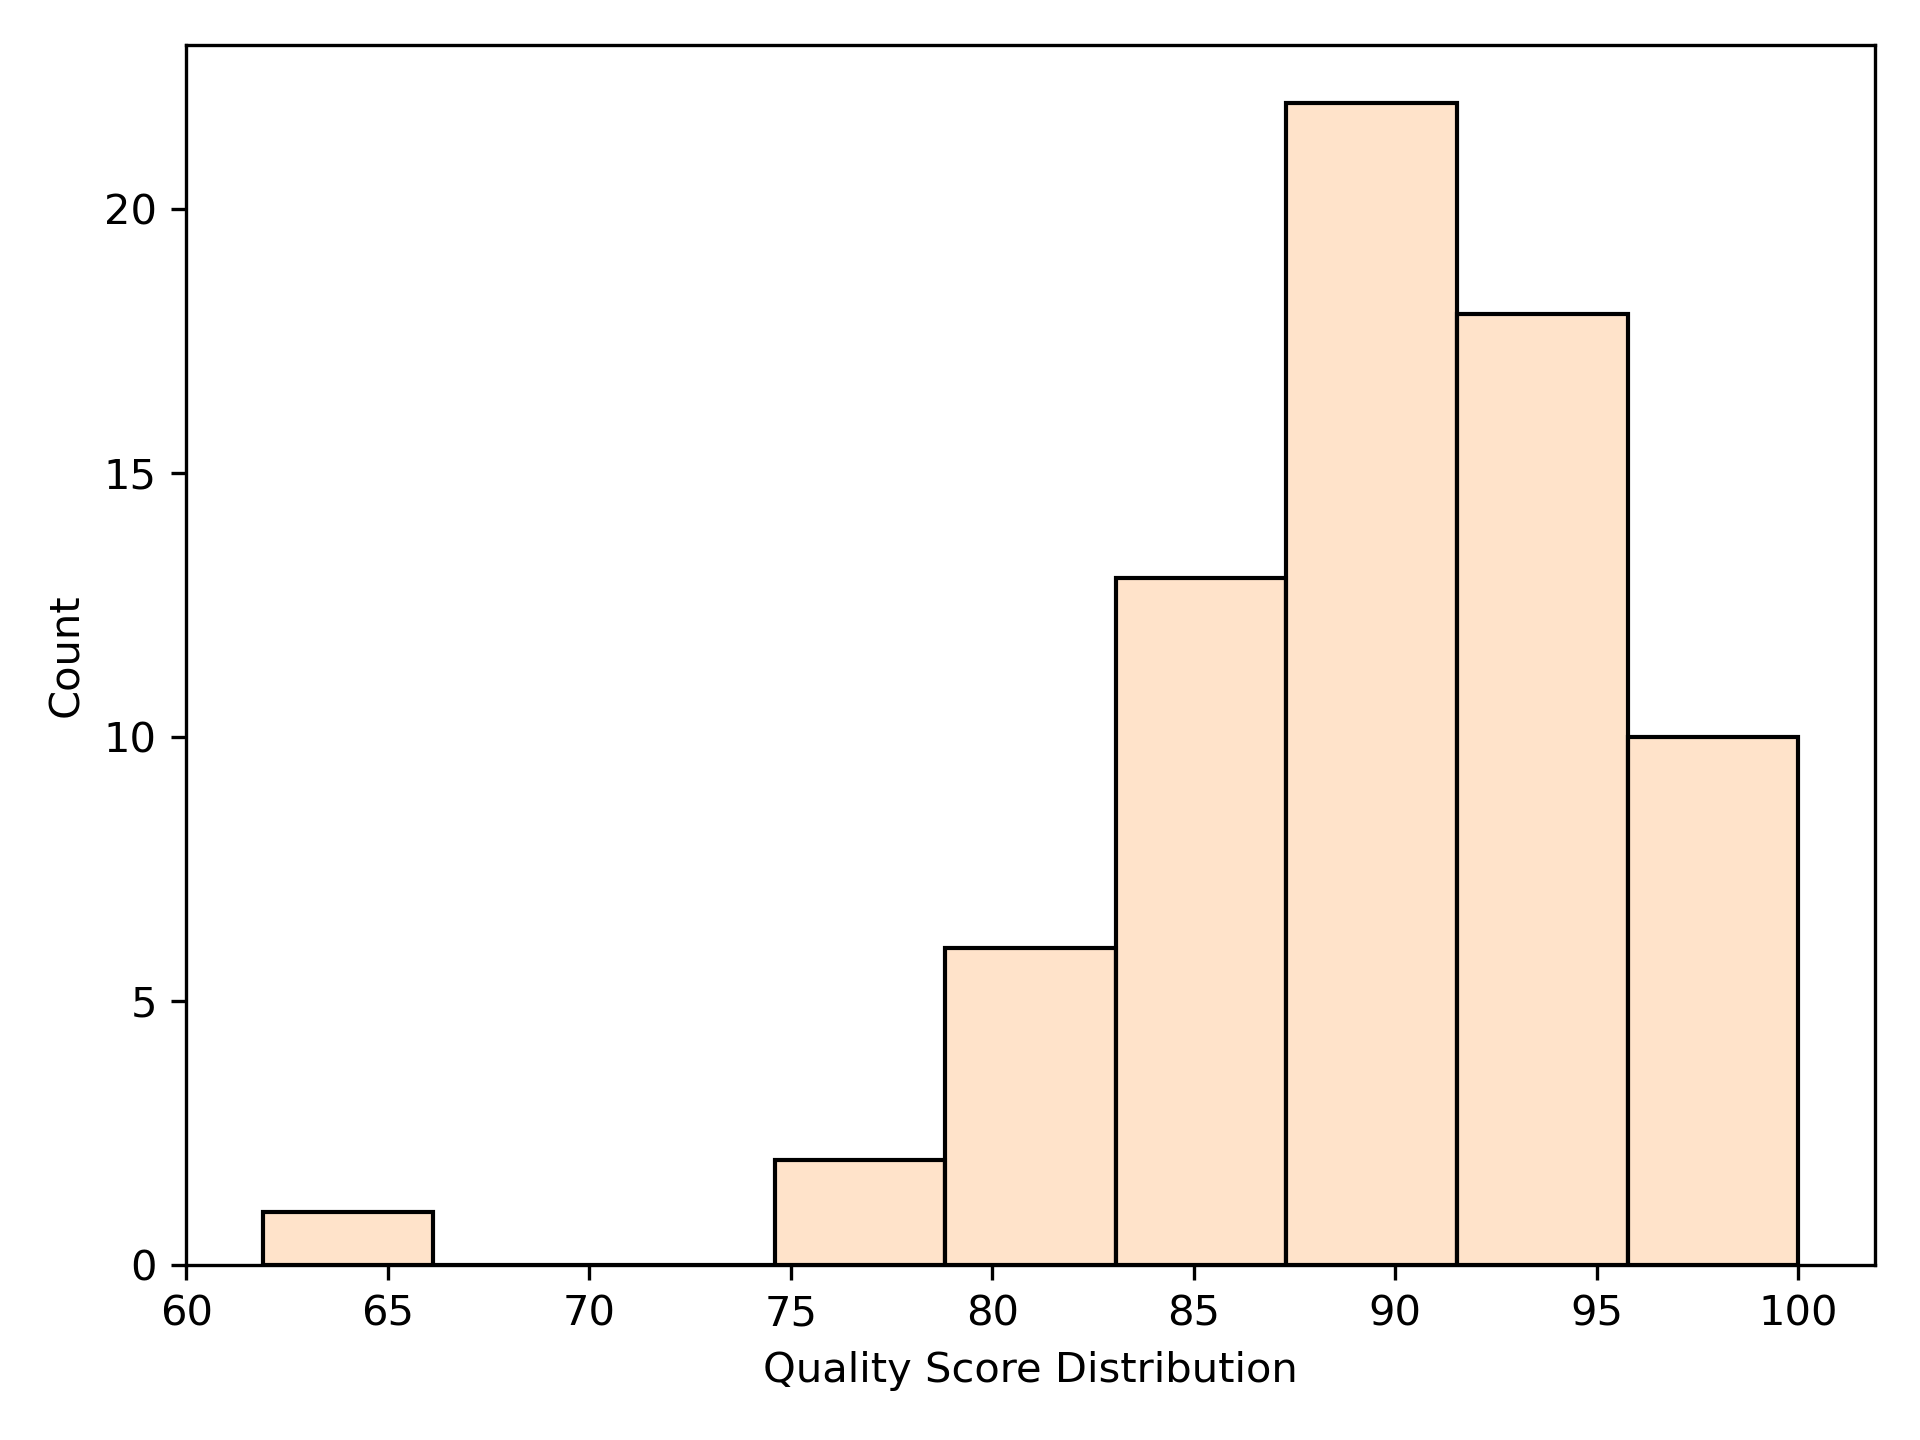
\includegraphics[width=\textwidth]{figs/qa_scores.png}
    \caption{Quality assessment score distribution for articles in the final subset.}
    \label{fig:qa_scores}
\end{figure}


\section{Quantitative Results}
\subsection{Querying Results}
Figures \ref{fig:bar_scopus} and \ref{fig:bar_wos} show quantitative querying results (the number of results per query combination) from Scopus and Web of Science as tree diagrams. 

\begin{figure}[ht!]
\centering
\begin{subfigure}{\textwidth}
    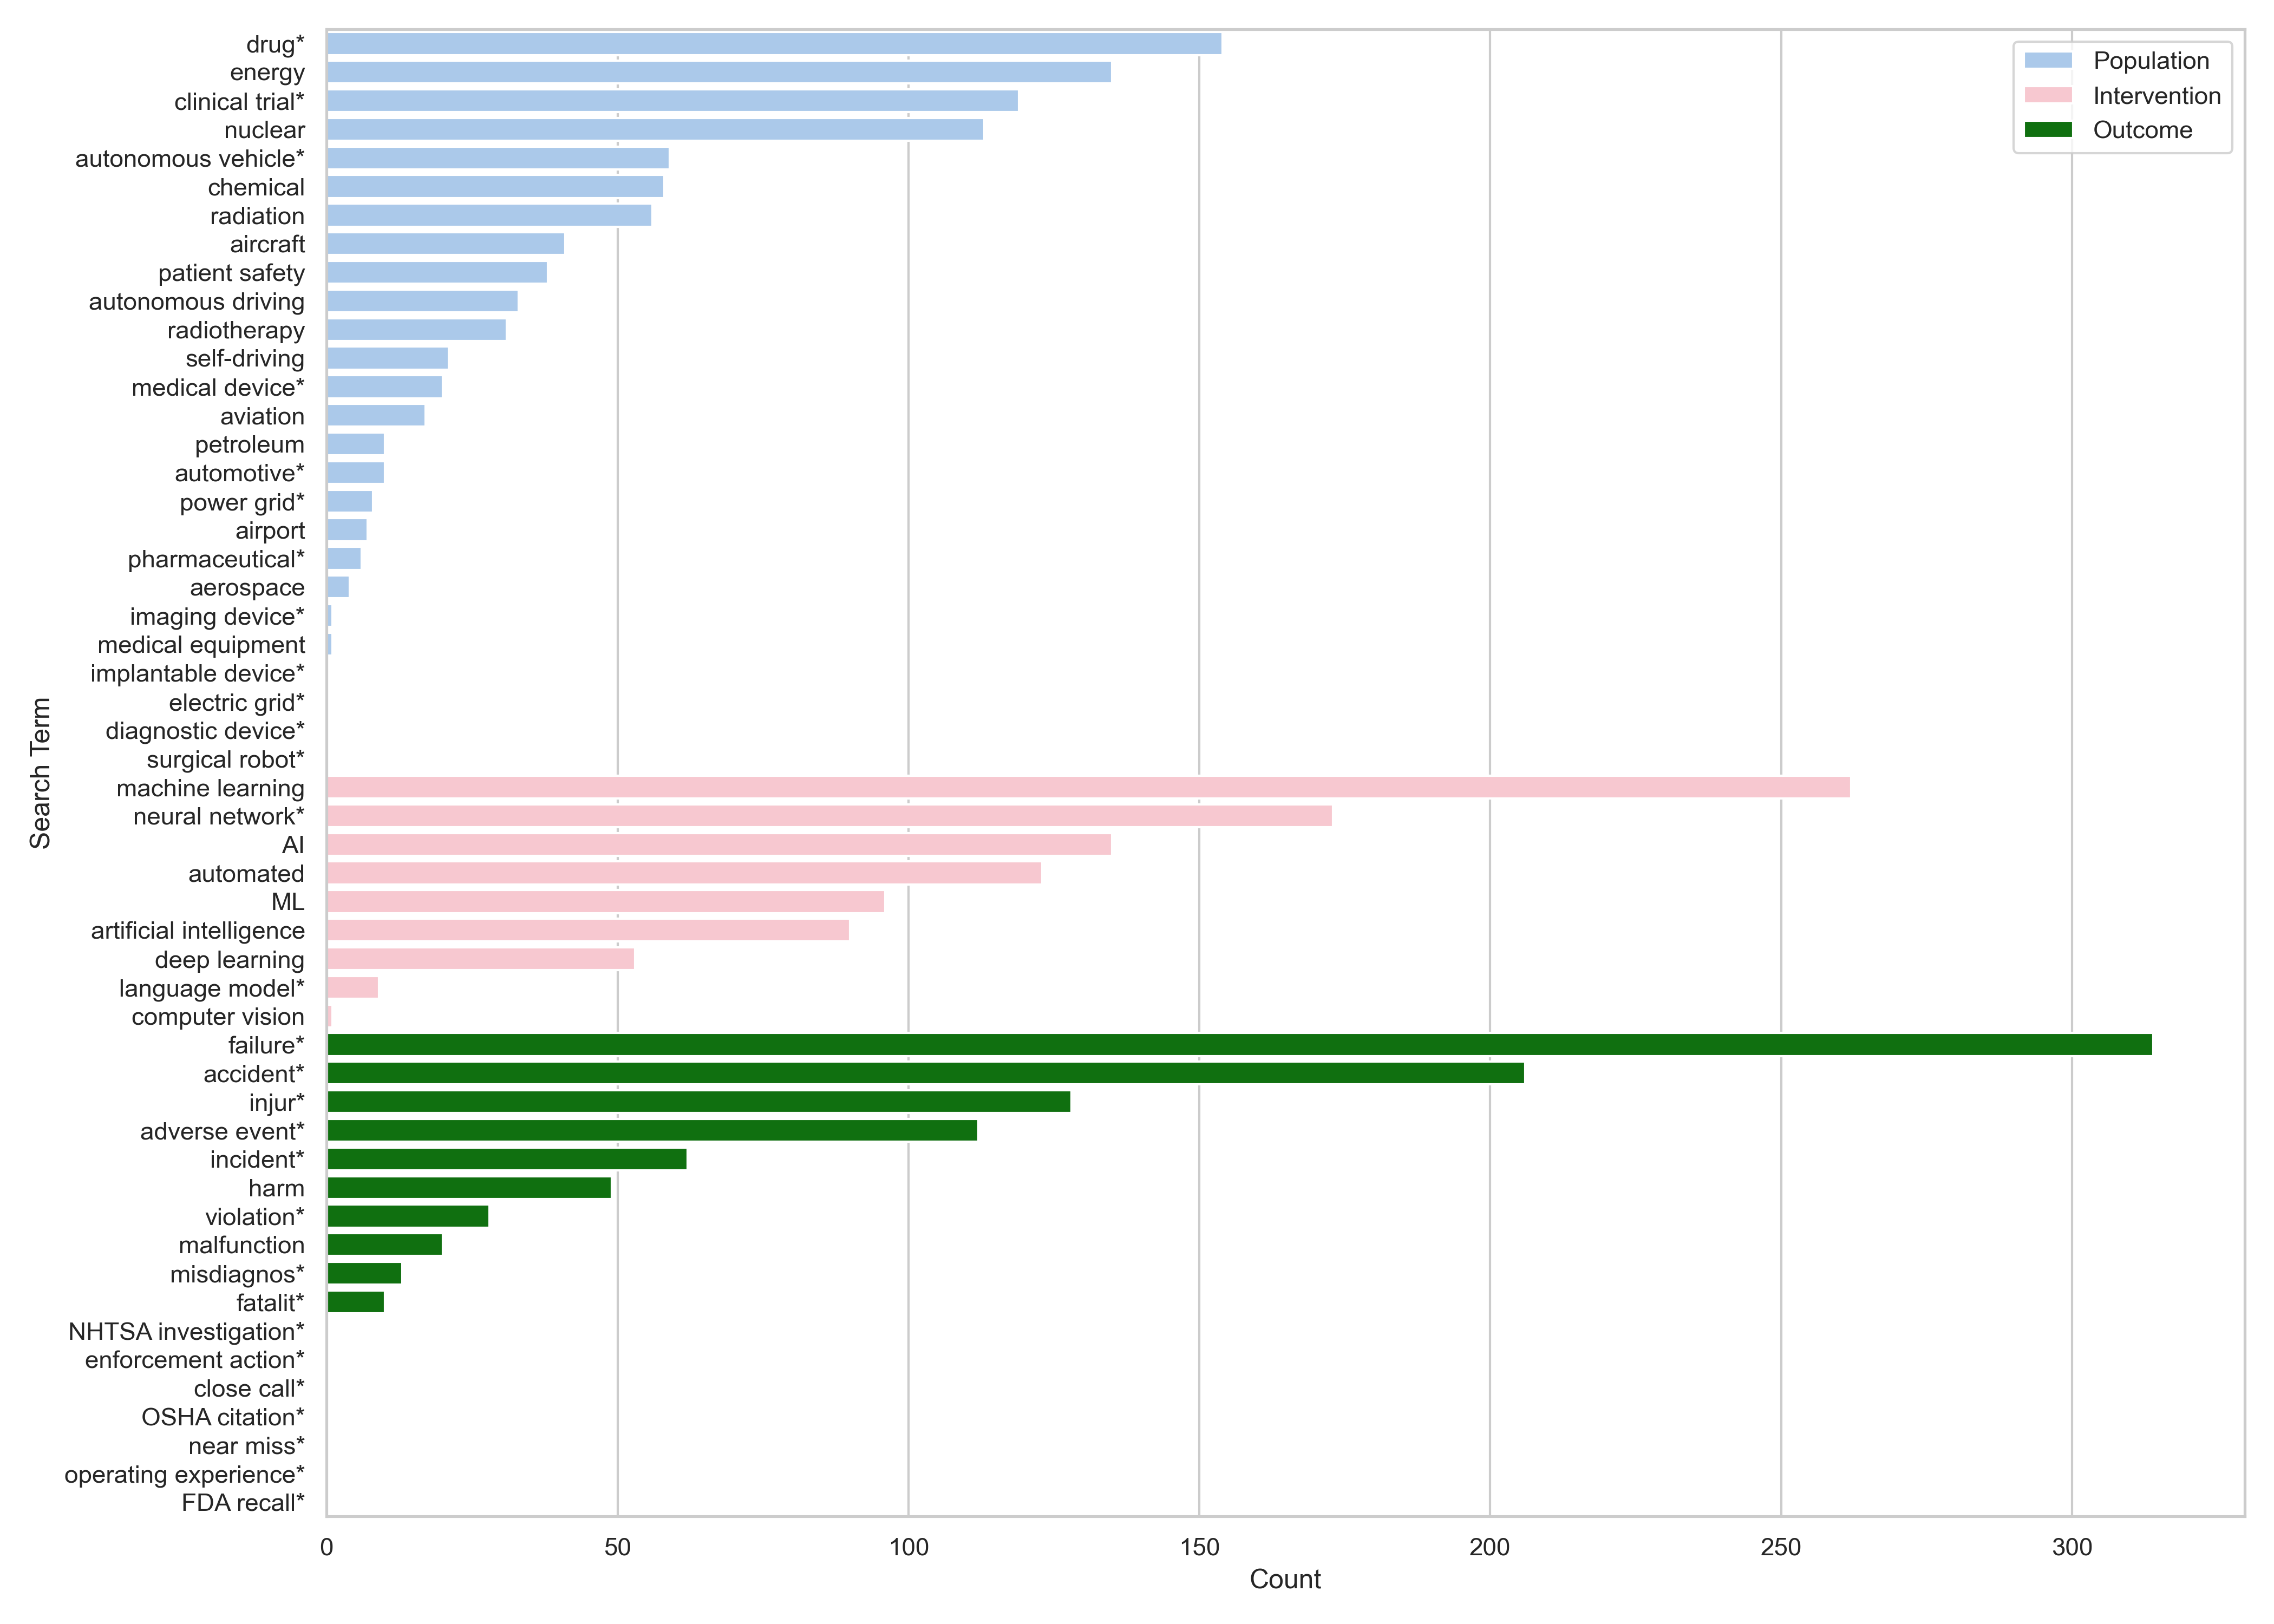
\includegraphics[width=\textwidth]{figs/bar_scopus.png}
    \caption{Scopus}
    \label{fig:bar_scopus}
\end{subfigure}
\hfill
\begin{subfigure}{\textwidth}
    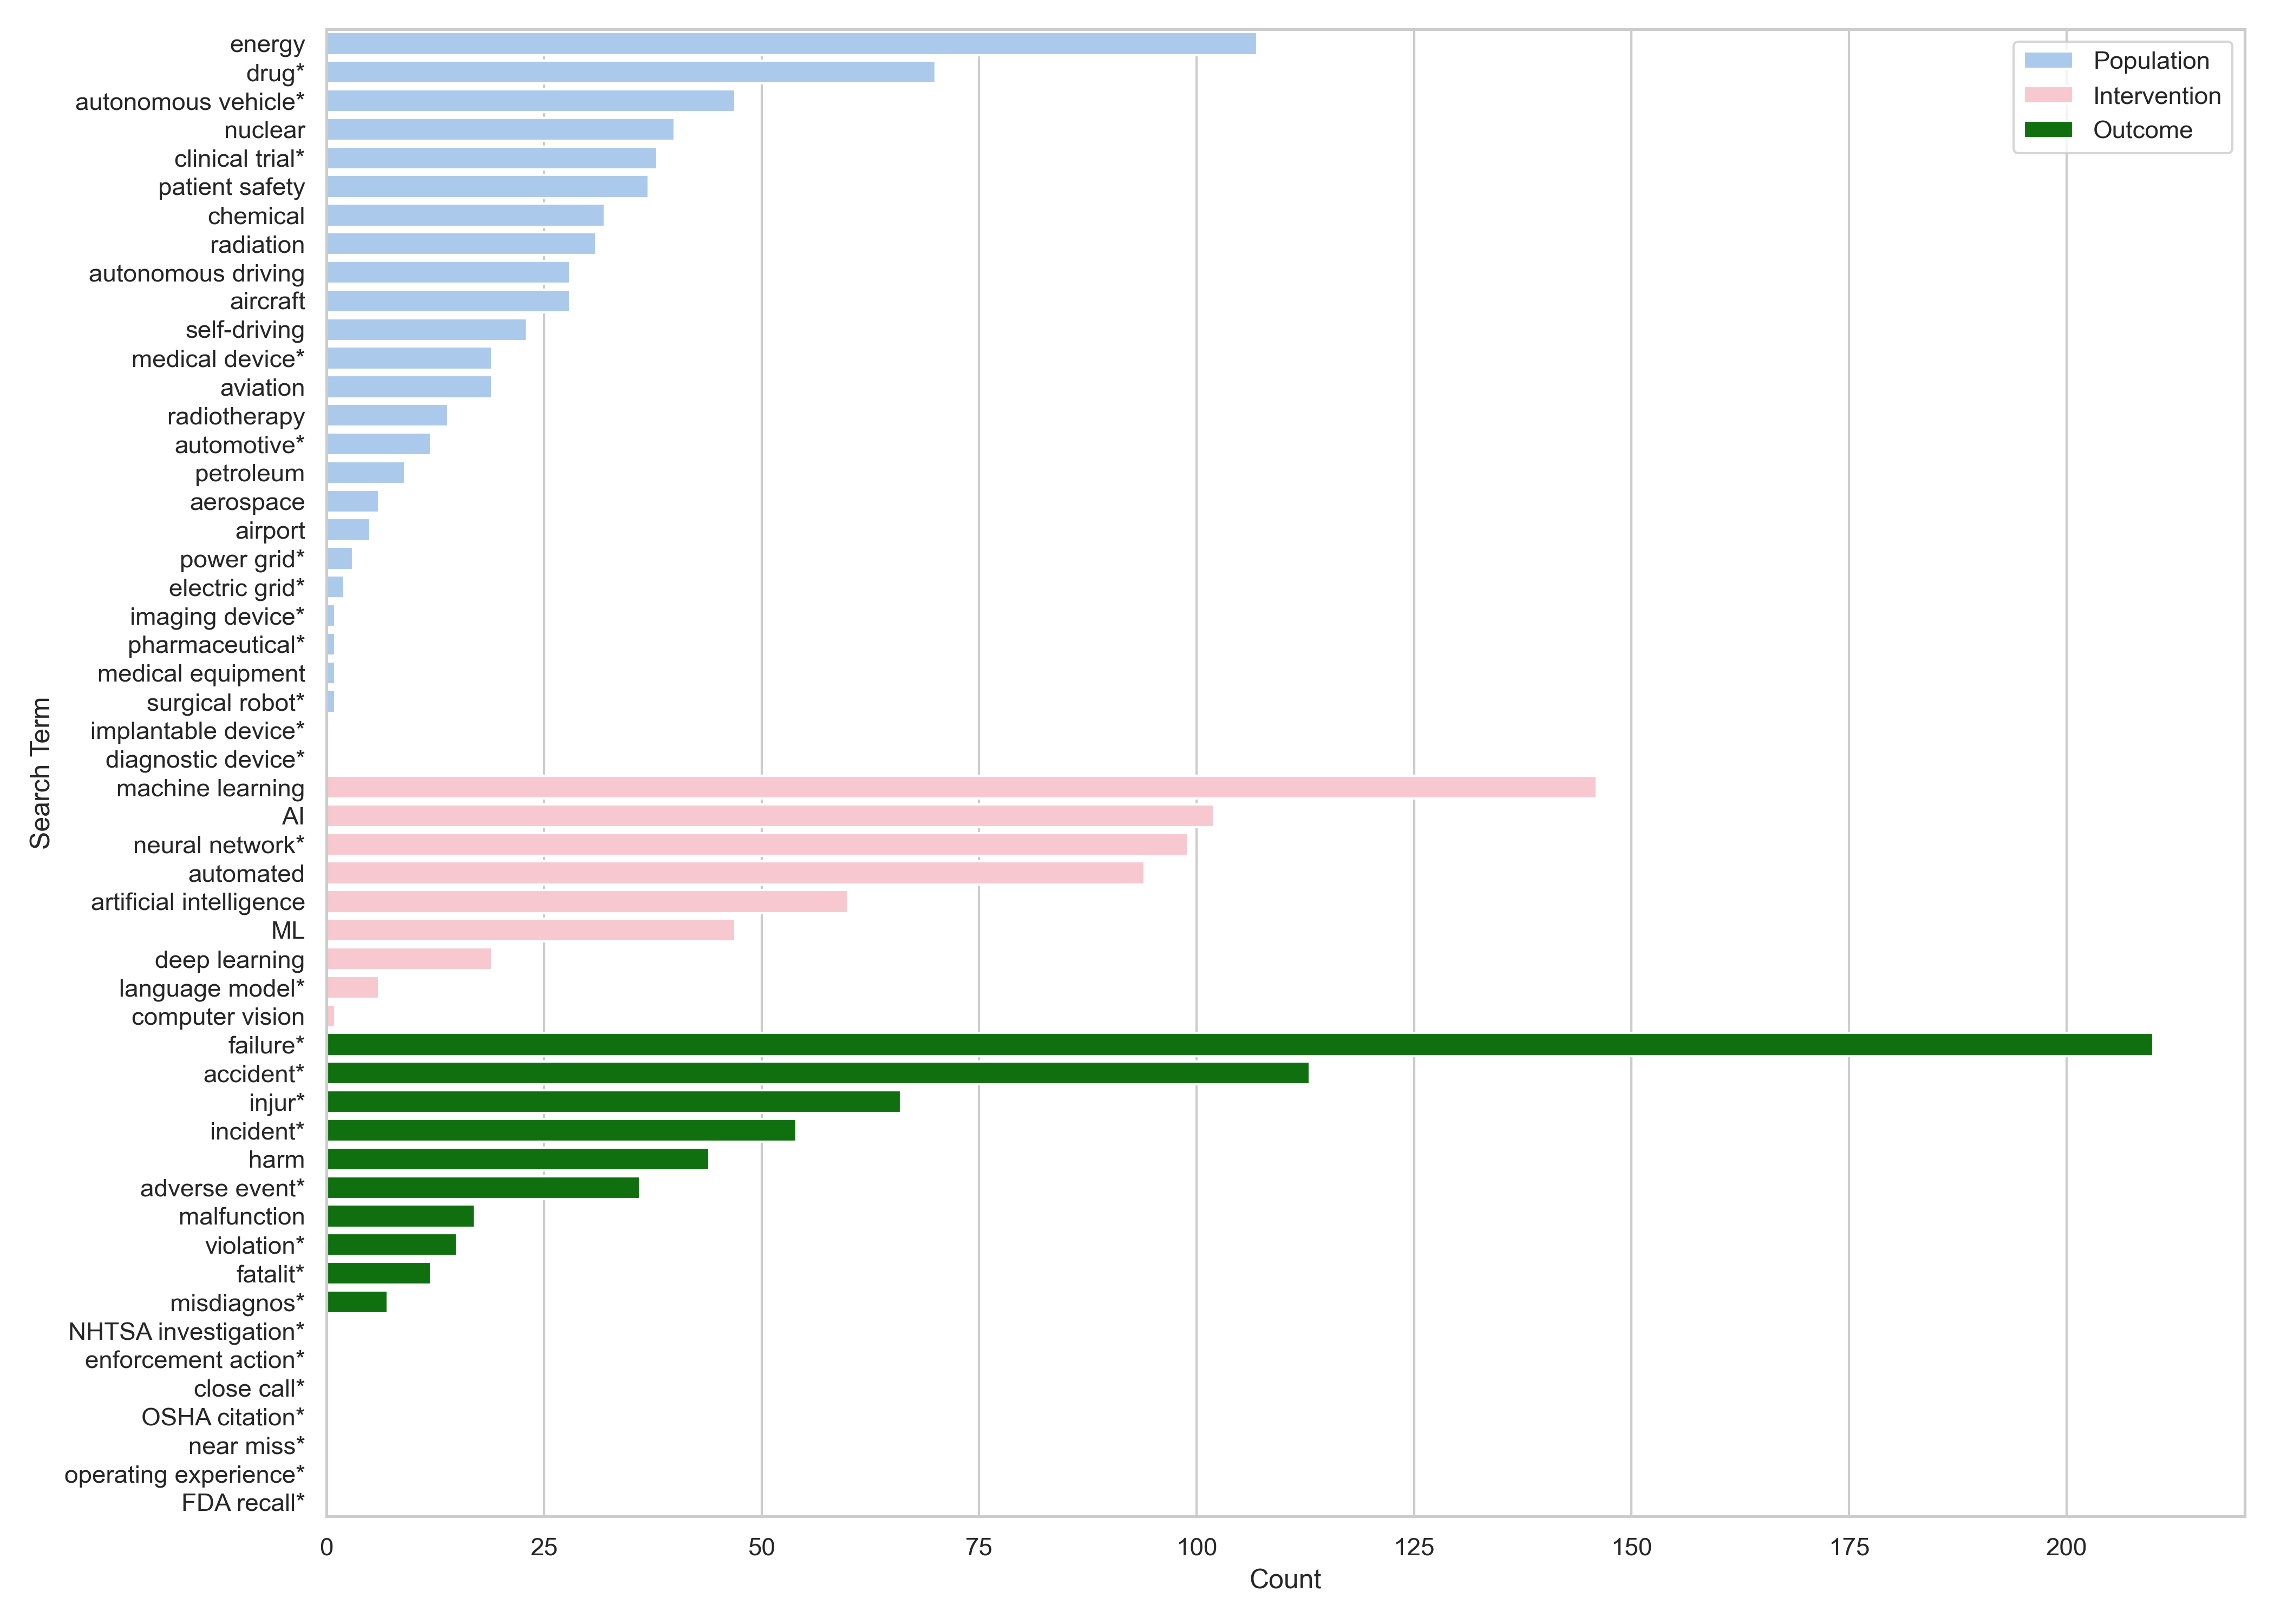
\includegraphics[width=\textwidth]{figs/bar_wos.png}
    \caption{Web of Science}
    \label{fig:bar_wos}
\end{subfigure}
Likewise, Figures \ref{fig:bar} shows the sum of articles returned by each Scopus and Web of Science when individual search terms were included in all queries.
\caption{Sum of articles returned by each database when a given search term was included in all queries.}
\label{fig:bar}
\end{figure}

\begin{figure}[ht!]
\centering
\begin{subfigure}{0.8\textwidth}
    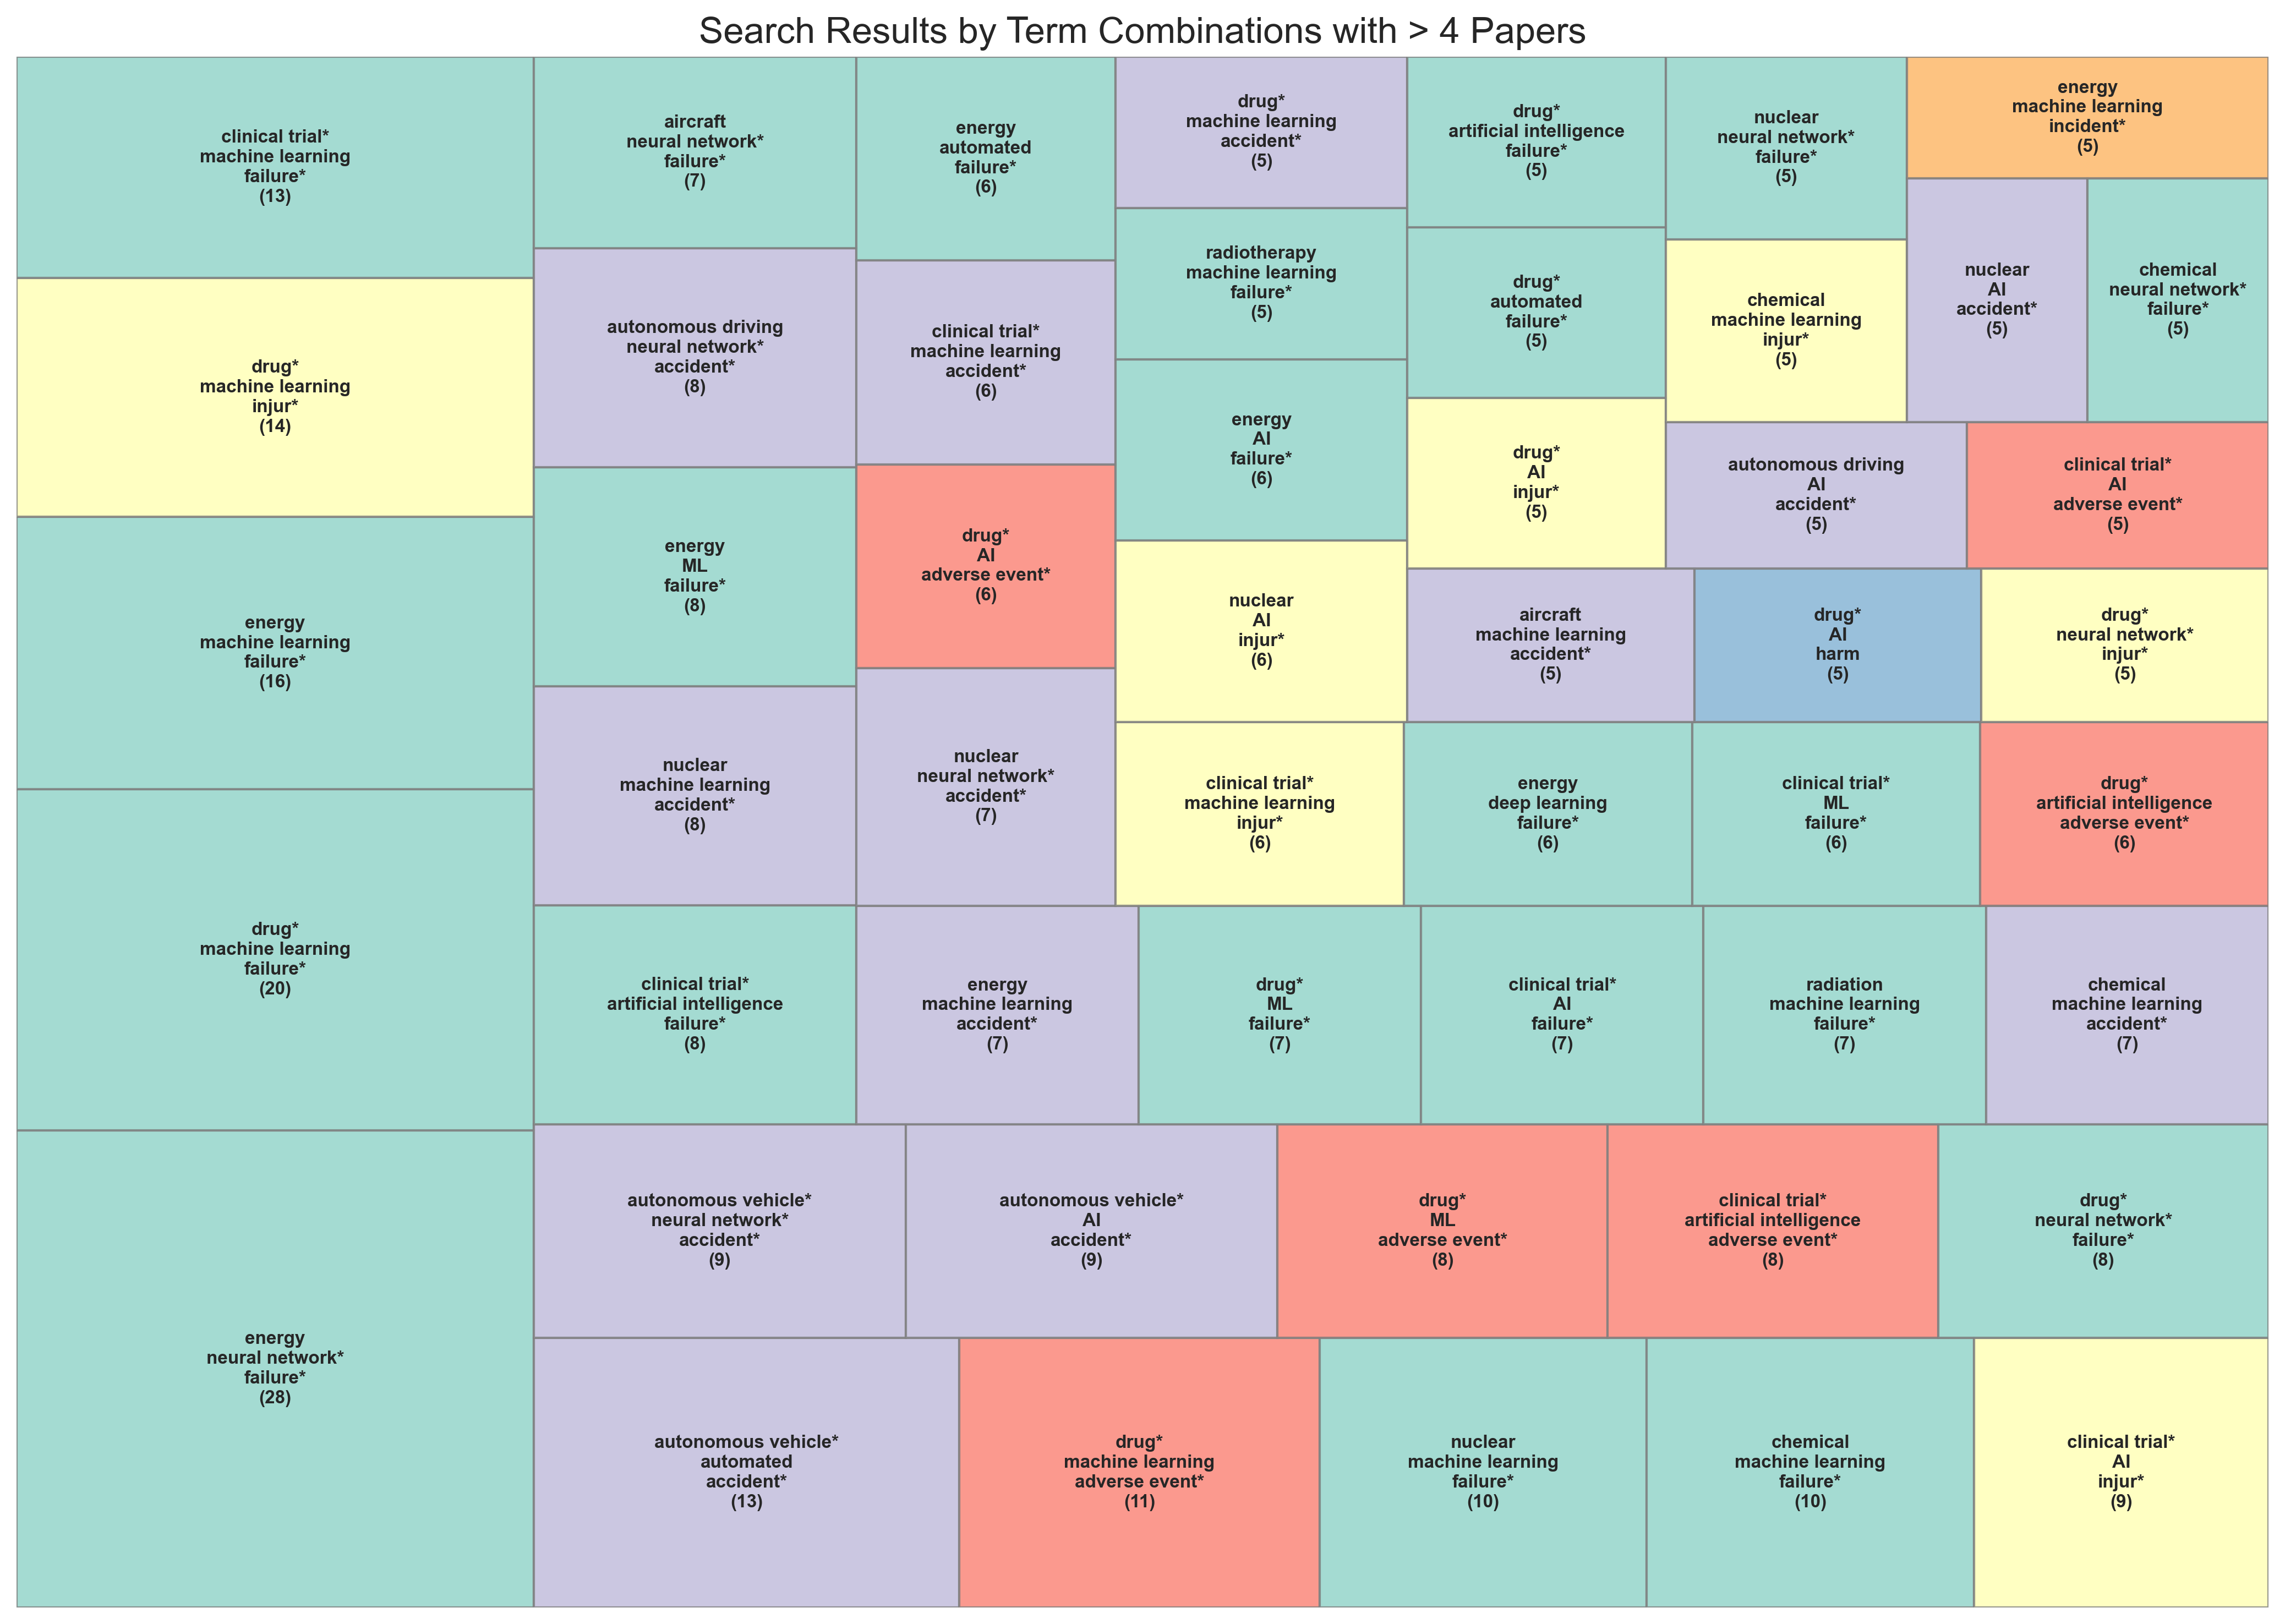
\includegraphics[width=\textwidth, trim=0cm 0cm 0cm 0.8cm, clip=true]{figs/large_tree_scopus.png}
    \caption{Scopus}
    \label{fig:tree_scopus}
\end{subfigure}
\hfill
\begin{subfigure}{0.8\textwidth}
    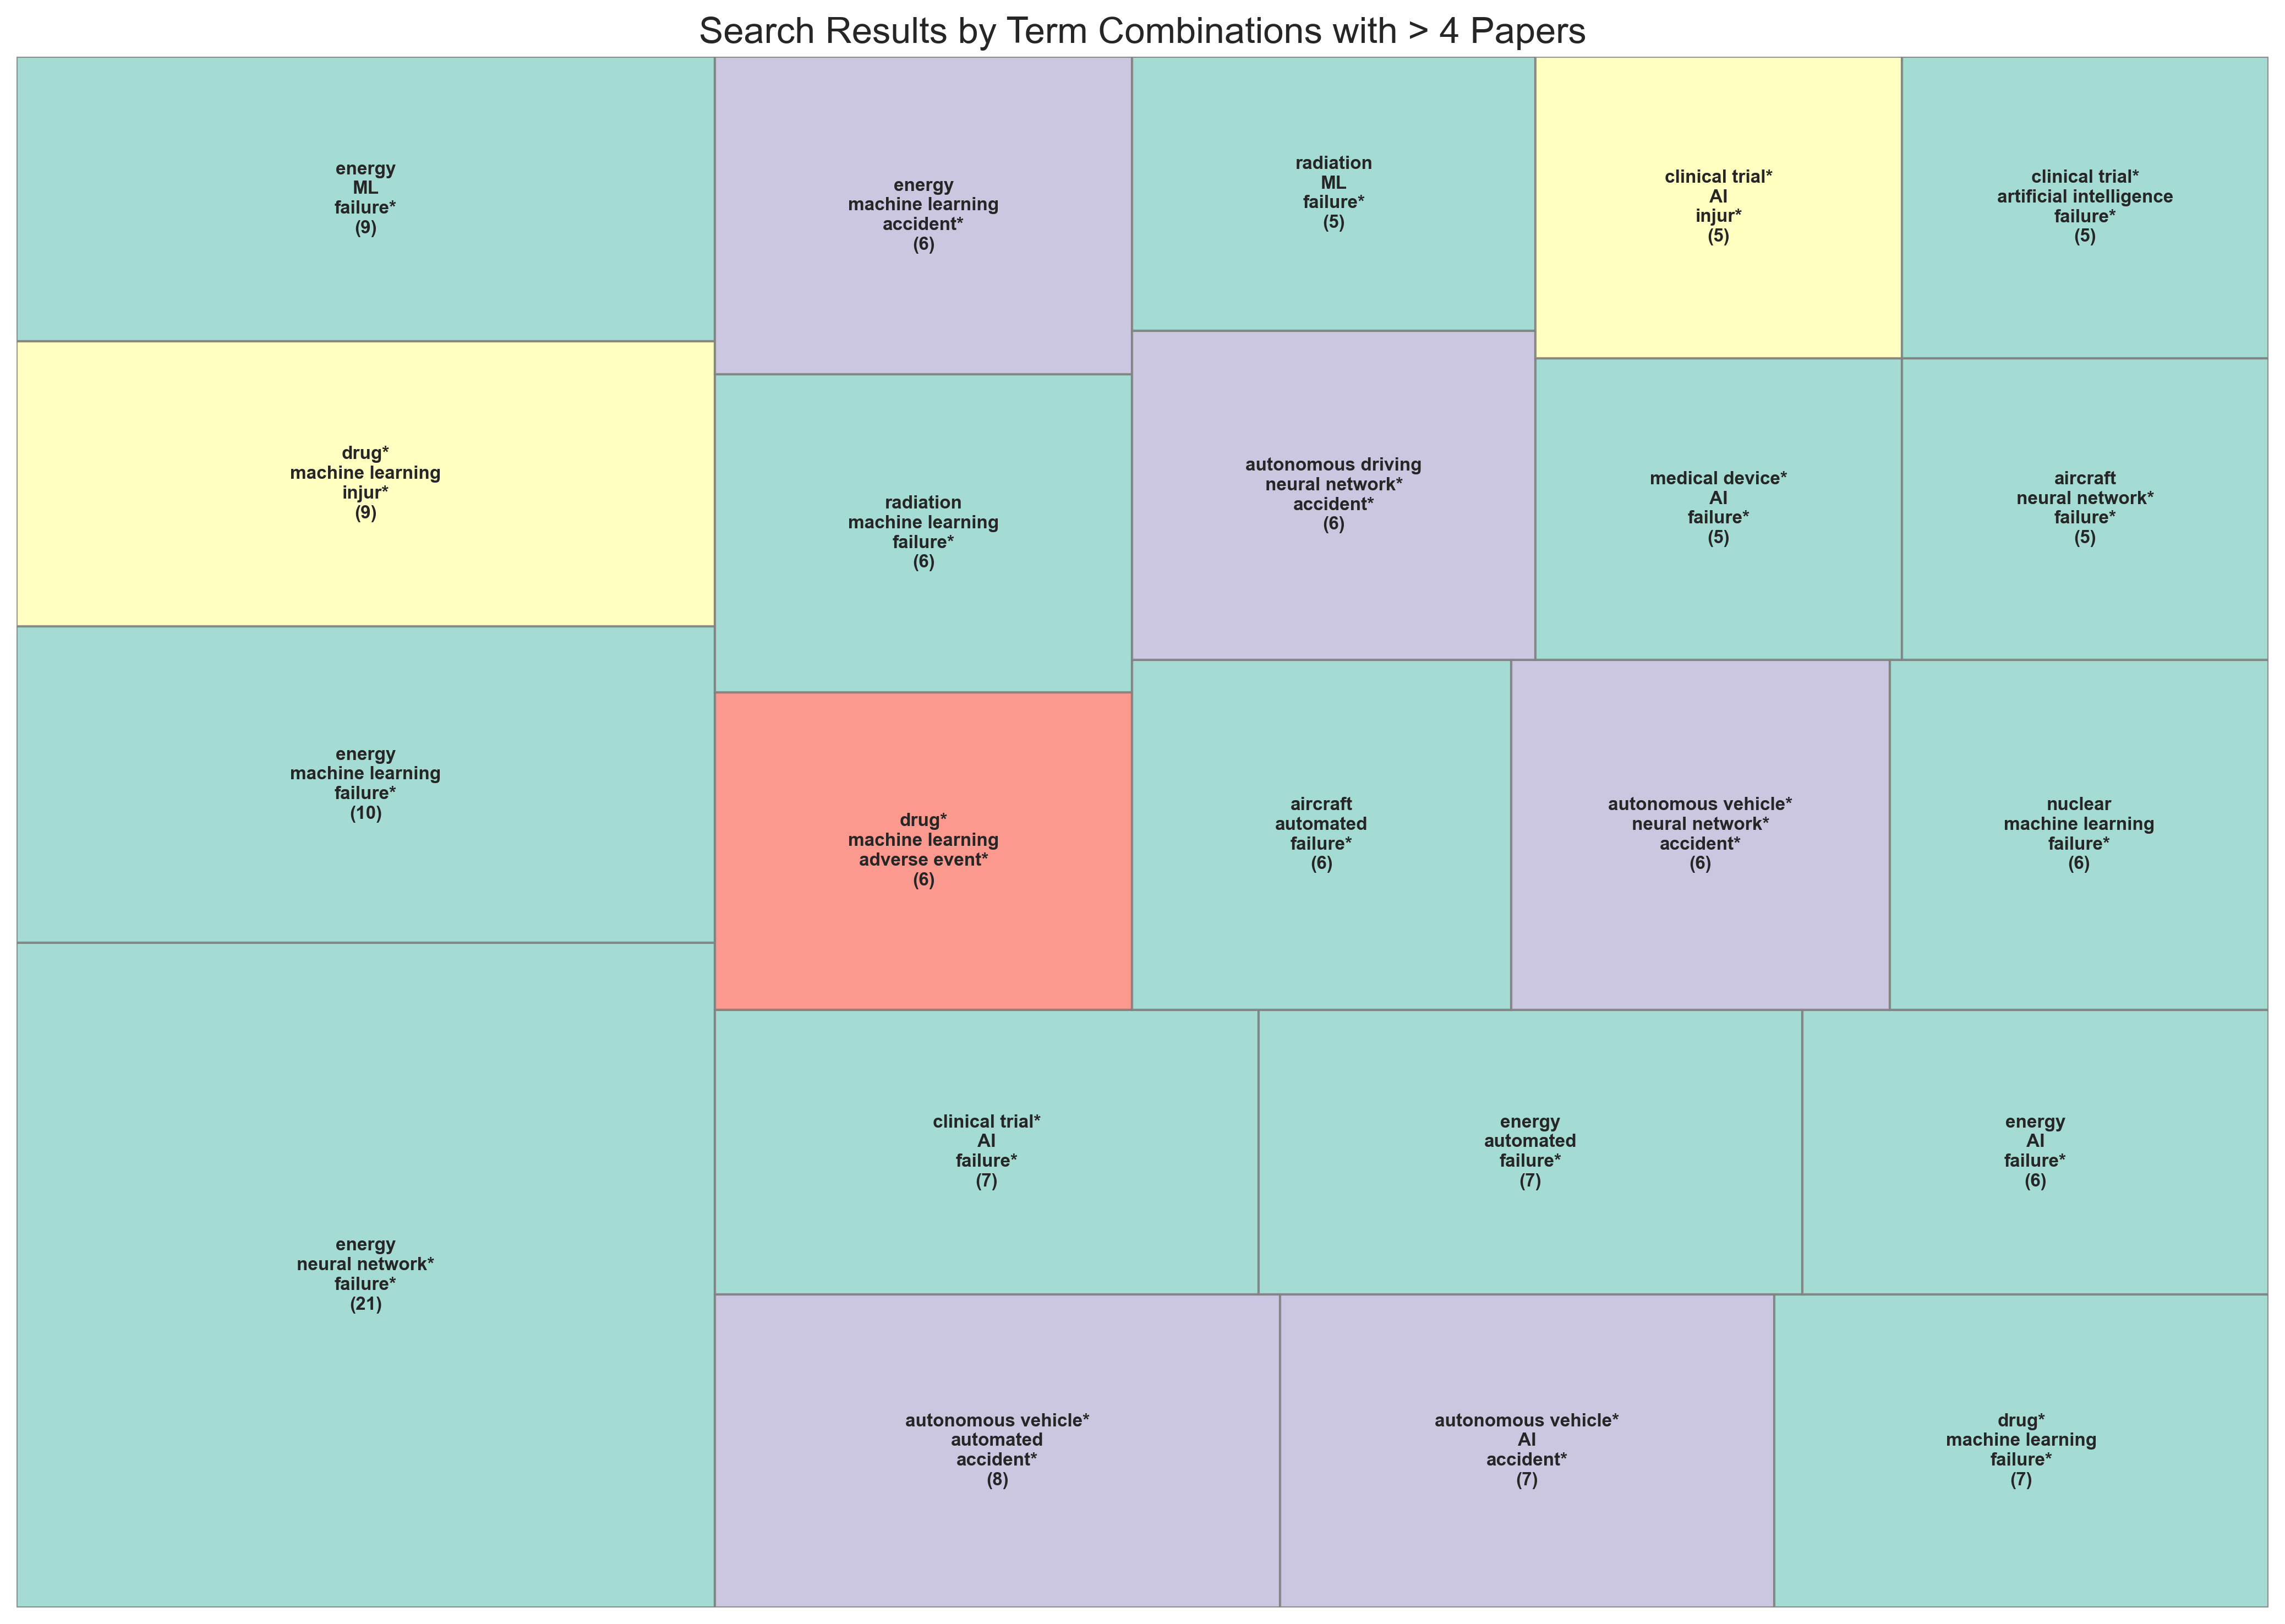
\includegraphics[width=\textwidth, trim=0cm 0cm 0cm 0.8cm, clip=true]{figs/large_tree_wos.png}
    \caption{Web of Science}
    \label{fig:tree_wos}
\end{subfigure}
       
\caption{Tree diagrams showing the sum of articles returned by each database for all query combinations that yielded $> 4$ results. Size of the box corresponds to the number of articles (also annotated) and color corresponds to outcome term.}
\label{fig:tree}
\end{figure}

\subsection{Data Extraction Results}
The database used to tabulate our results can be accessed \href{https://www.notion.so/2ff683956c2580a9b1cdcf750b987f70?v=0b1df89639f442c29749d75c23802f13&source=copy_link}{here.} \textcolor{red}{Additionally, we provide a database in Supplemental Materials.}

After extracting the information mentioned in \ref{sec:methods}, we created a variety of figures to portray key trends from the set of articles reviewed. This includes country of author institution, main AI type considered in the article, decision-making type, whether regulation or explainability was considered, and types of explainability methods considered. 

% AI Method
Figure \ref{fig:ai_type} shows the number of articles that employed each type of AI in the final subset of articles. Note that many articles employed more than one type of AI, so Figure \ref{fig:ai_type} shows more counts than total articles. Similarly, some articles focused on ethical or regulatory frameworks and therefore considered AI more generally. We denote the AI type in these articles as ``Non-Specific.''

\begin{figure}[ht!]
    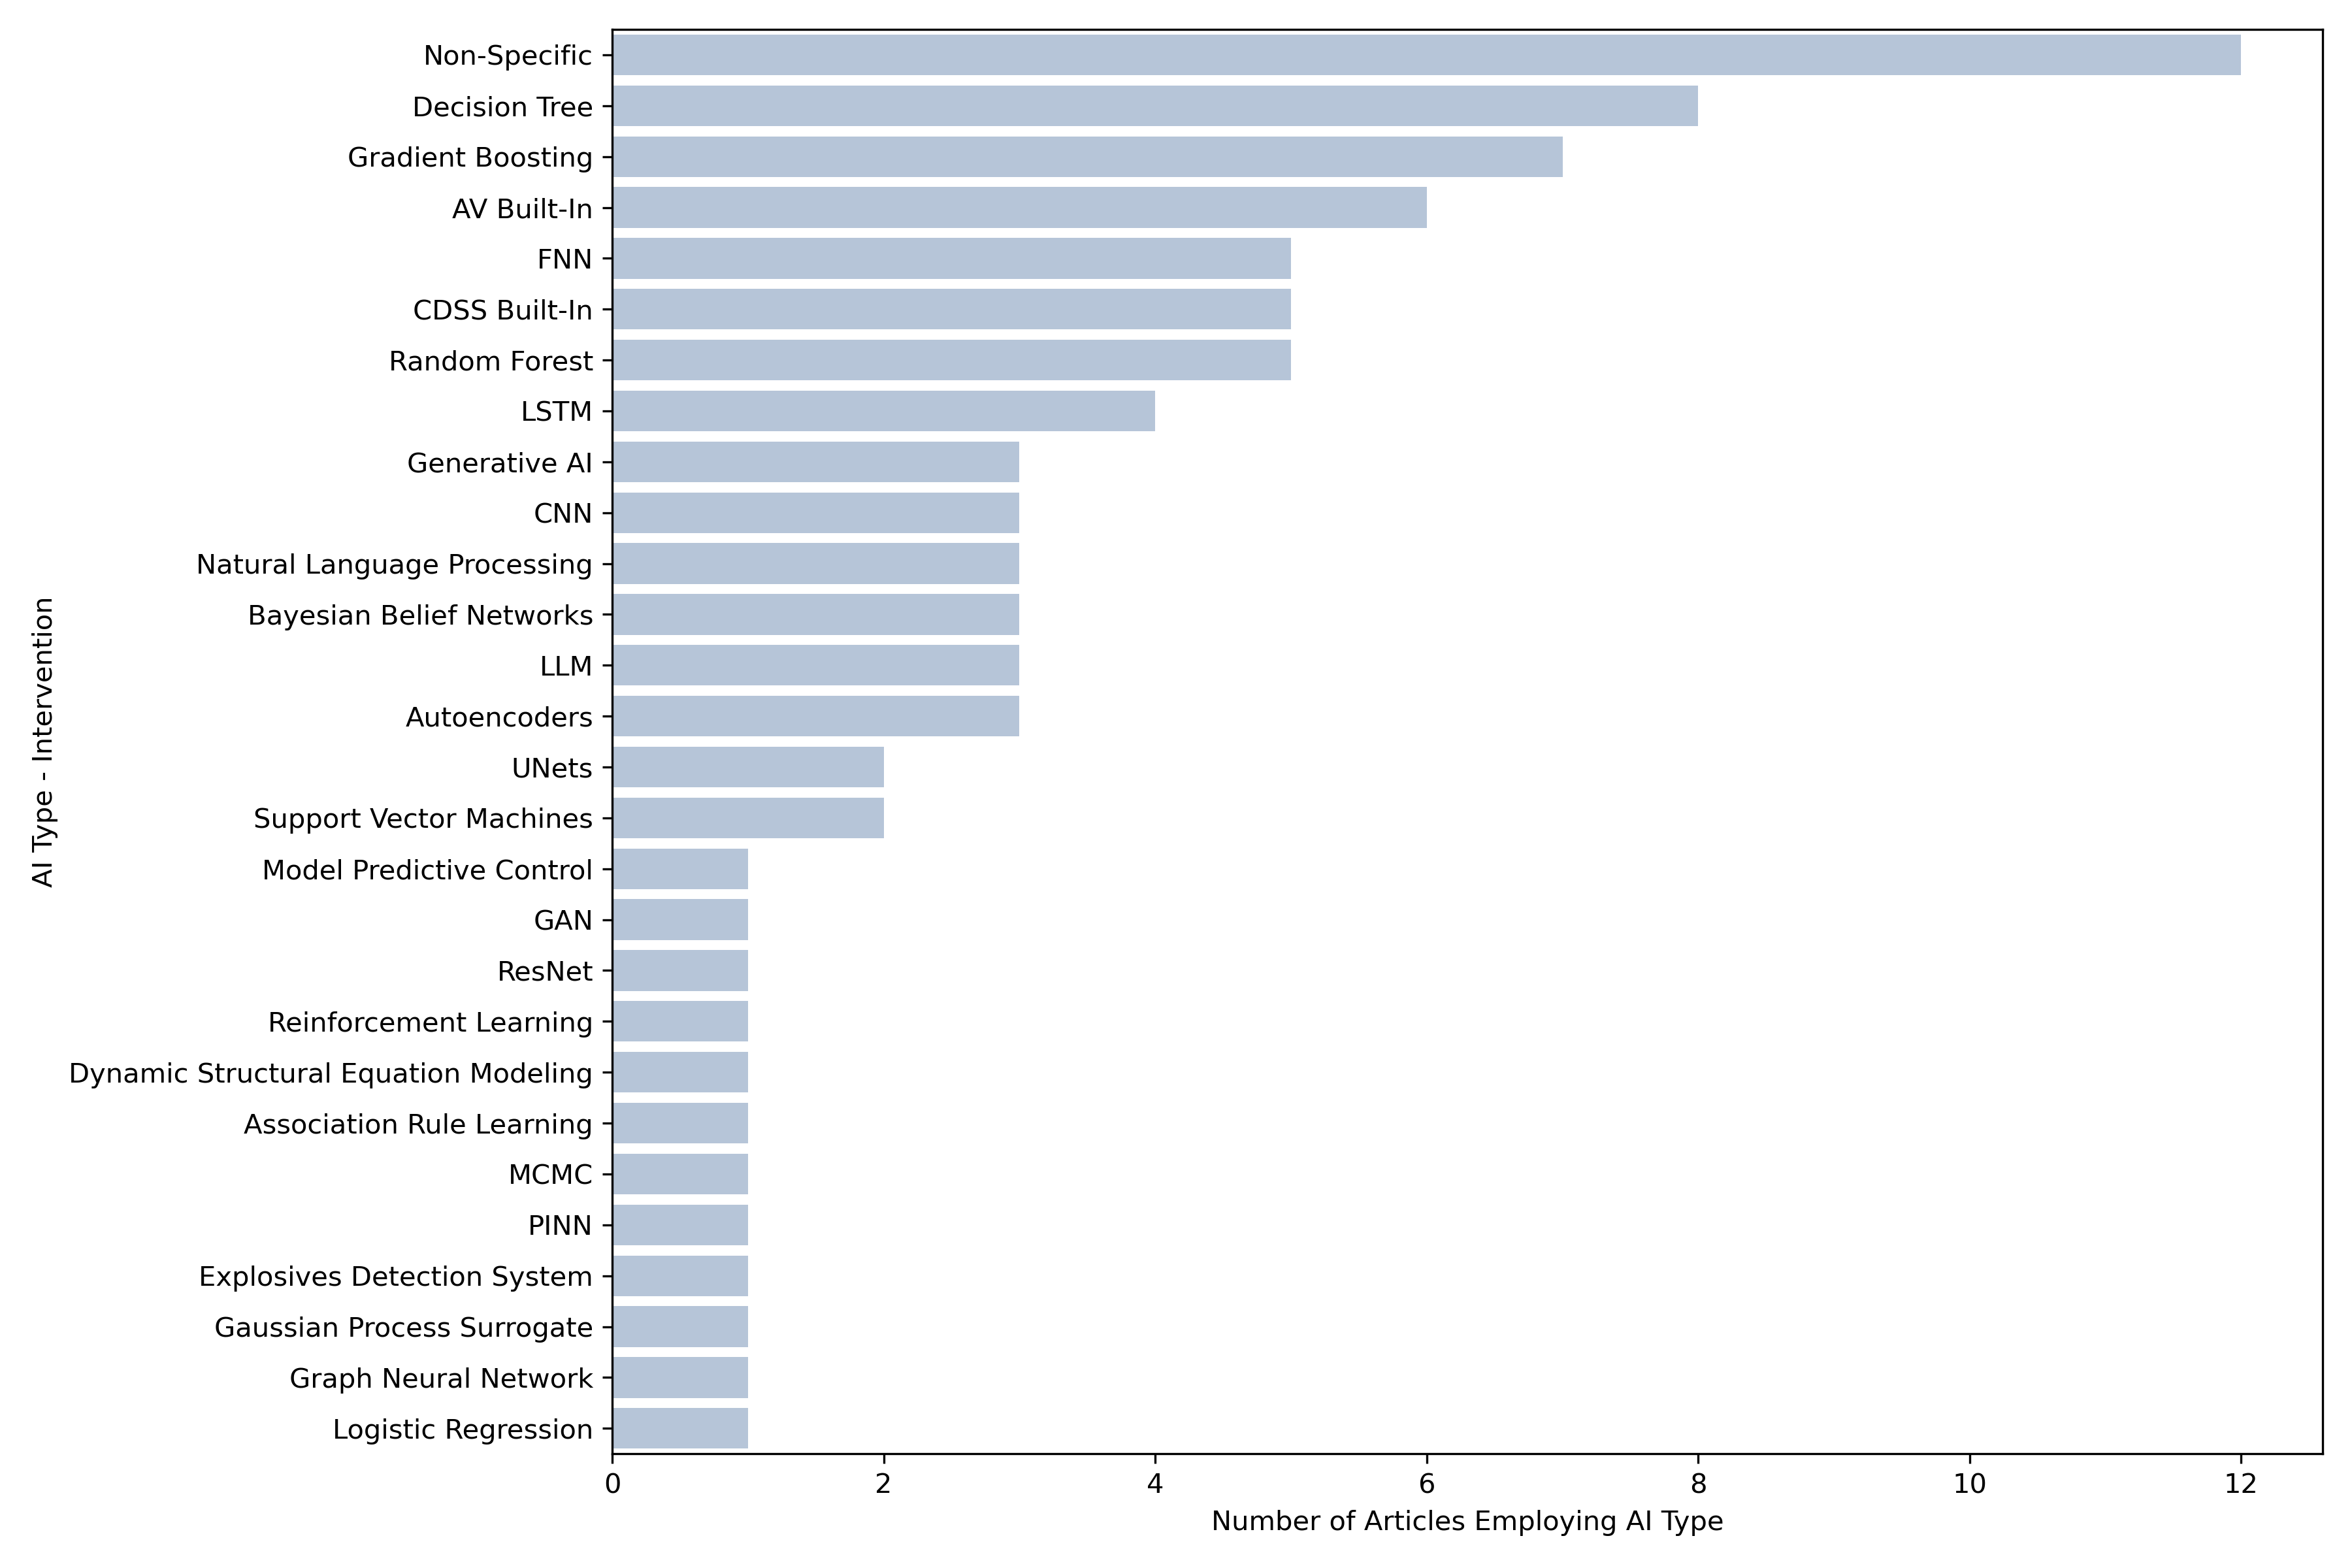
\includegraphics[width=\textwidth]{figs/ai_type.png}
    \caption{Number of articles in final subset that considered each type of AI method. Non-specific means the article did not provide details about the model type.}
    \label{fig:ai_type}
\end{figure}

% Decision Making Method
Figure \ref{fig:dm_type} shows the decision-making type evaluated by the articles in the final subset. ``Not system integrated'' refers to articles that use AI to set some kind of threshold or benchmark value for decision-making, but do not actually integrate a dynamic version of the AI itself into the system under consideration. Additionally, we distinguish ``augmented human decision-making'' and ``human in the loop'' as systems that both require human action to make decisions, but human in the loop leans more heavily on the AI system whereas augmented simply uses the AI results as an additional piece of information to make a decision with. Autonomous systems do not necessarily require human oversight to take action, though they may have it for intervention purposes. This type of system is most typical with autonomous vehicles. 

\begin{figure}[ht!]
    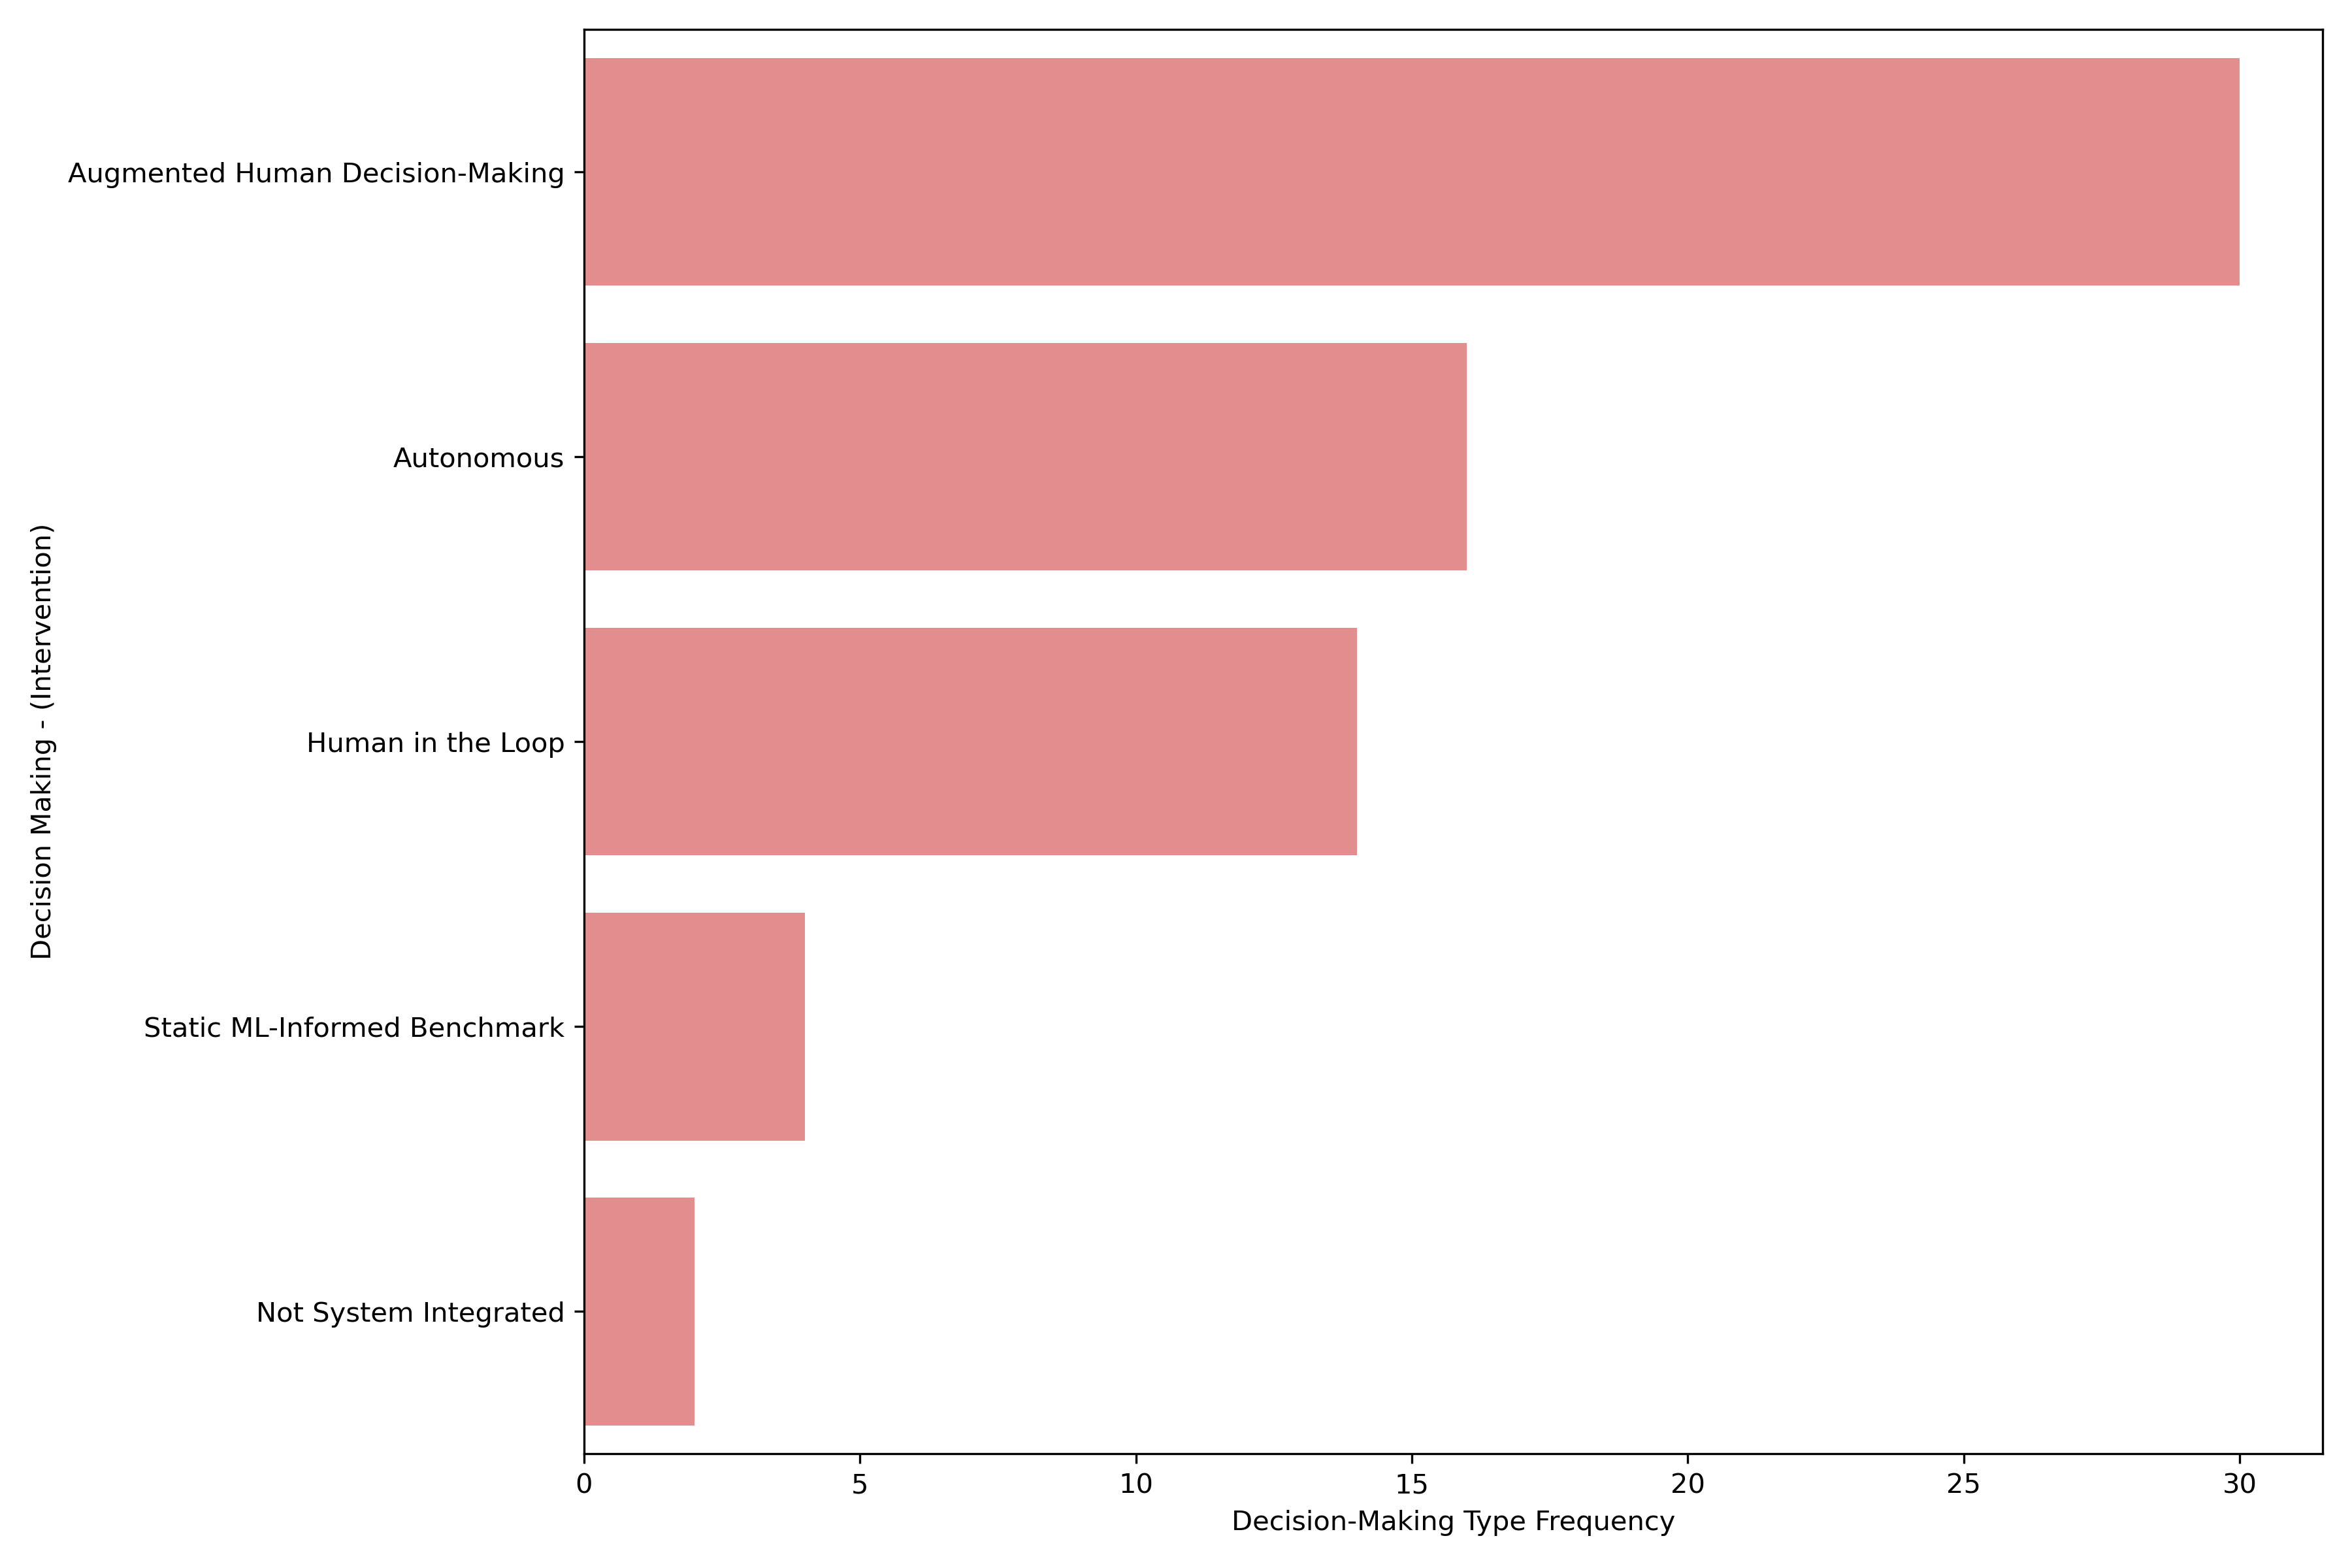
\includegraphics[width=\textwidth]{figs/dm_type.png}
    \caption{Decision-making types observed in final article subset.}
    \label{fig:dm_type}
\end{figure}

% Explanation Method
Approximately 49\% of the articles in our final subset considered explanation methods in some capacity. Of those that did, Figure \ref{fig:explain_type} shows which explanation method they employed. In some instances, authors mentioned the importance of explainability, therefore considering it, but did not conduct any explainability analysis themselves. These articles were denoted a ``Non-Specific'' explainability type in Figure \ref{fig:explain_type}.

\begin{figure}[ht!]
    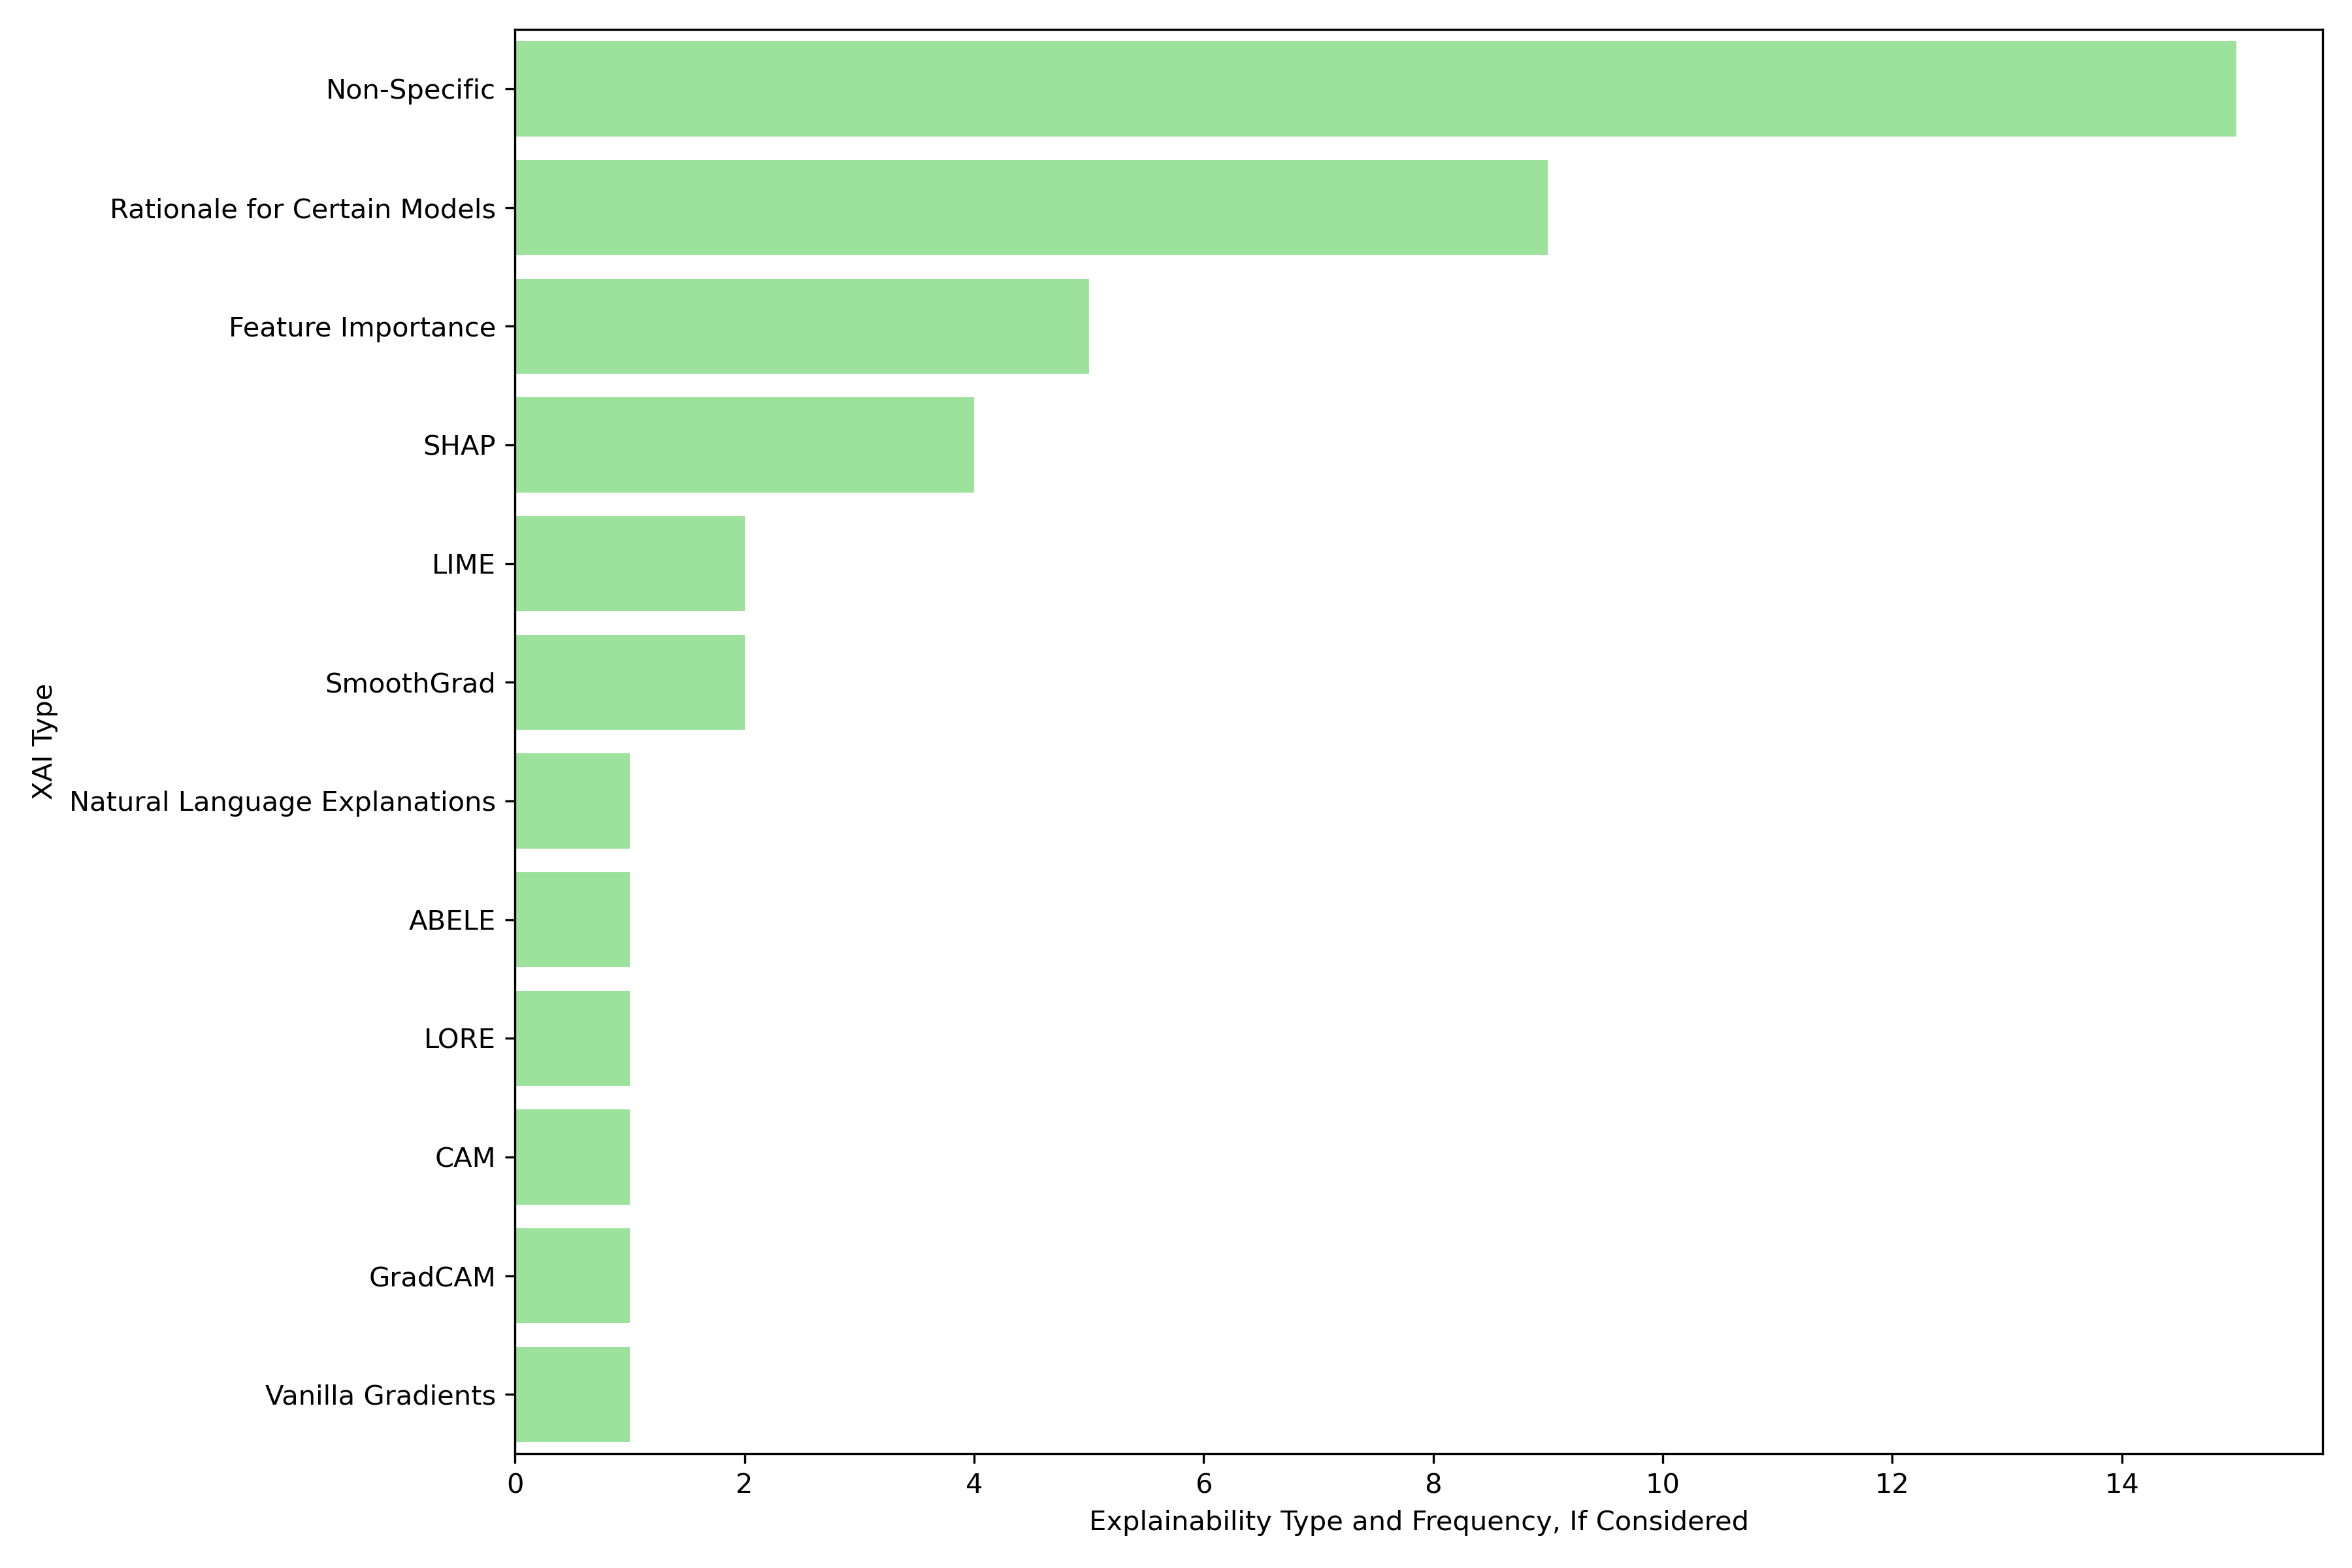
\includegraphics[width=\textwidth]{figs/explain_type.png}
    \caption{Explanation types observed in final article subset. ``Non-Specific'' indicates that explainability was considered but no method was applied.}
    \label{fig:explain_type}
\end{figure}

% Country of Origin
Figures \ref{fig:country} and \ref{fig:country_map} show the number of articles who have at least one contributing author from the countries shown. Of the final subset of articles, approximately 44\% considered regulatory oversight. This distribution of countries is therefore intended to show how the regulatory oversight bodies might be distributed and to highlight the complexity of defining AI regulatory frameworks that span international boundaries. 

\begin{figure}[ht!]
    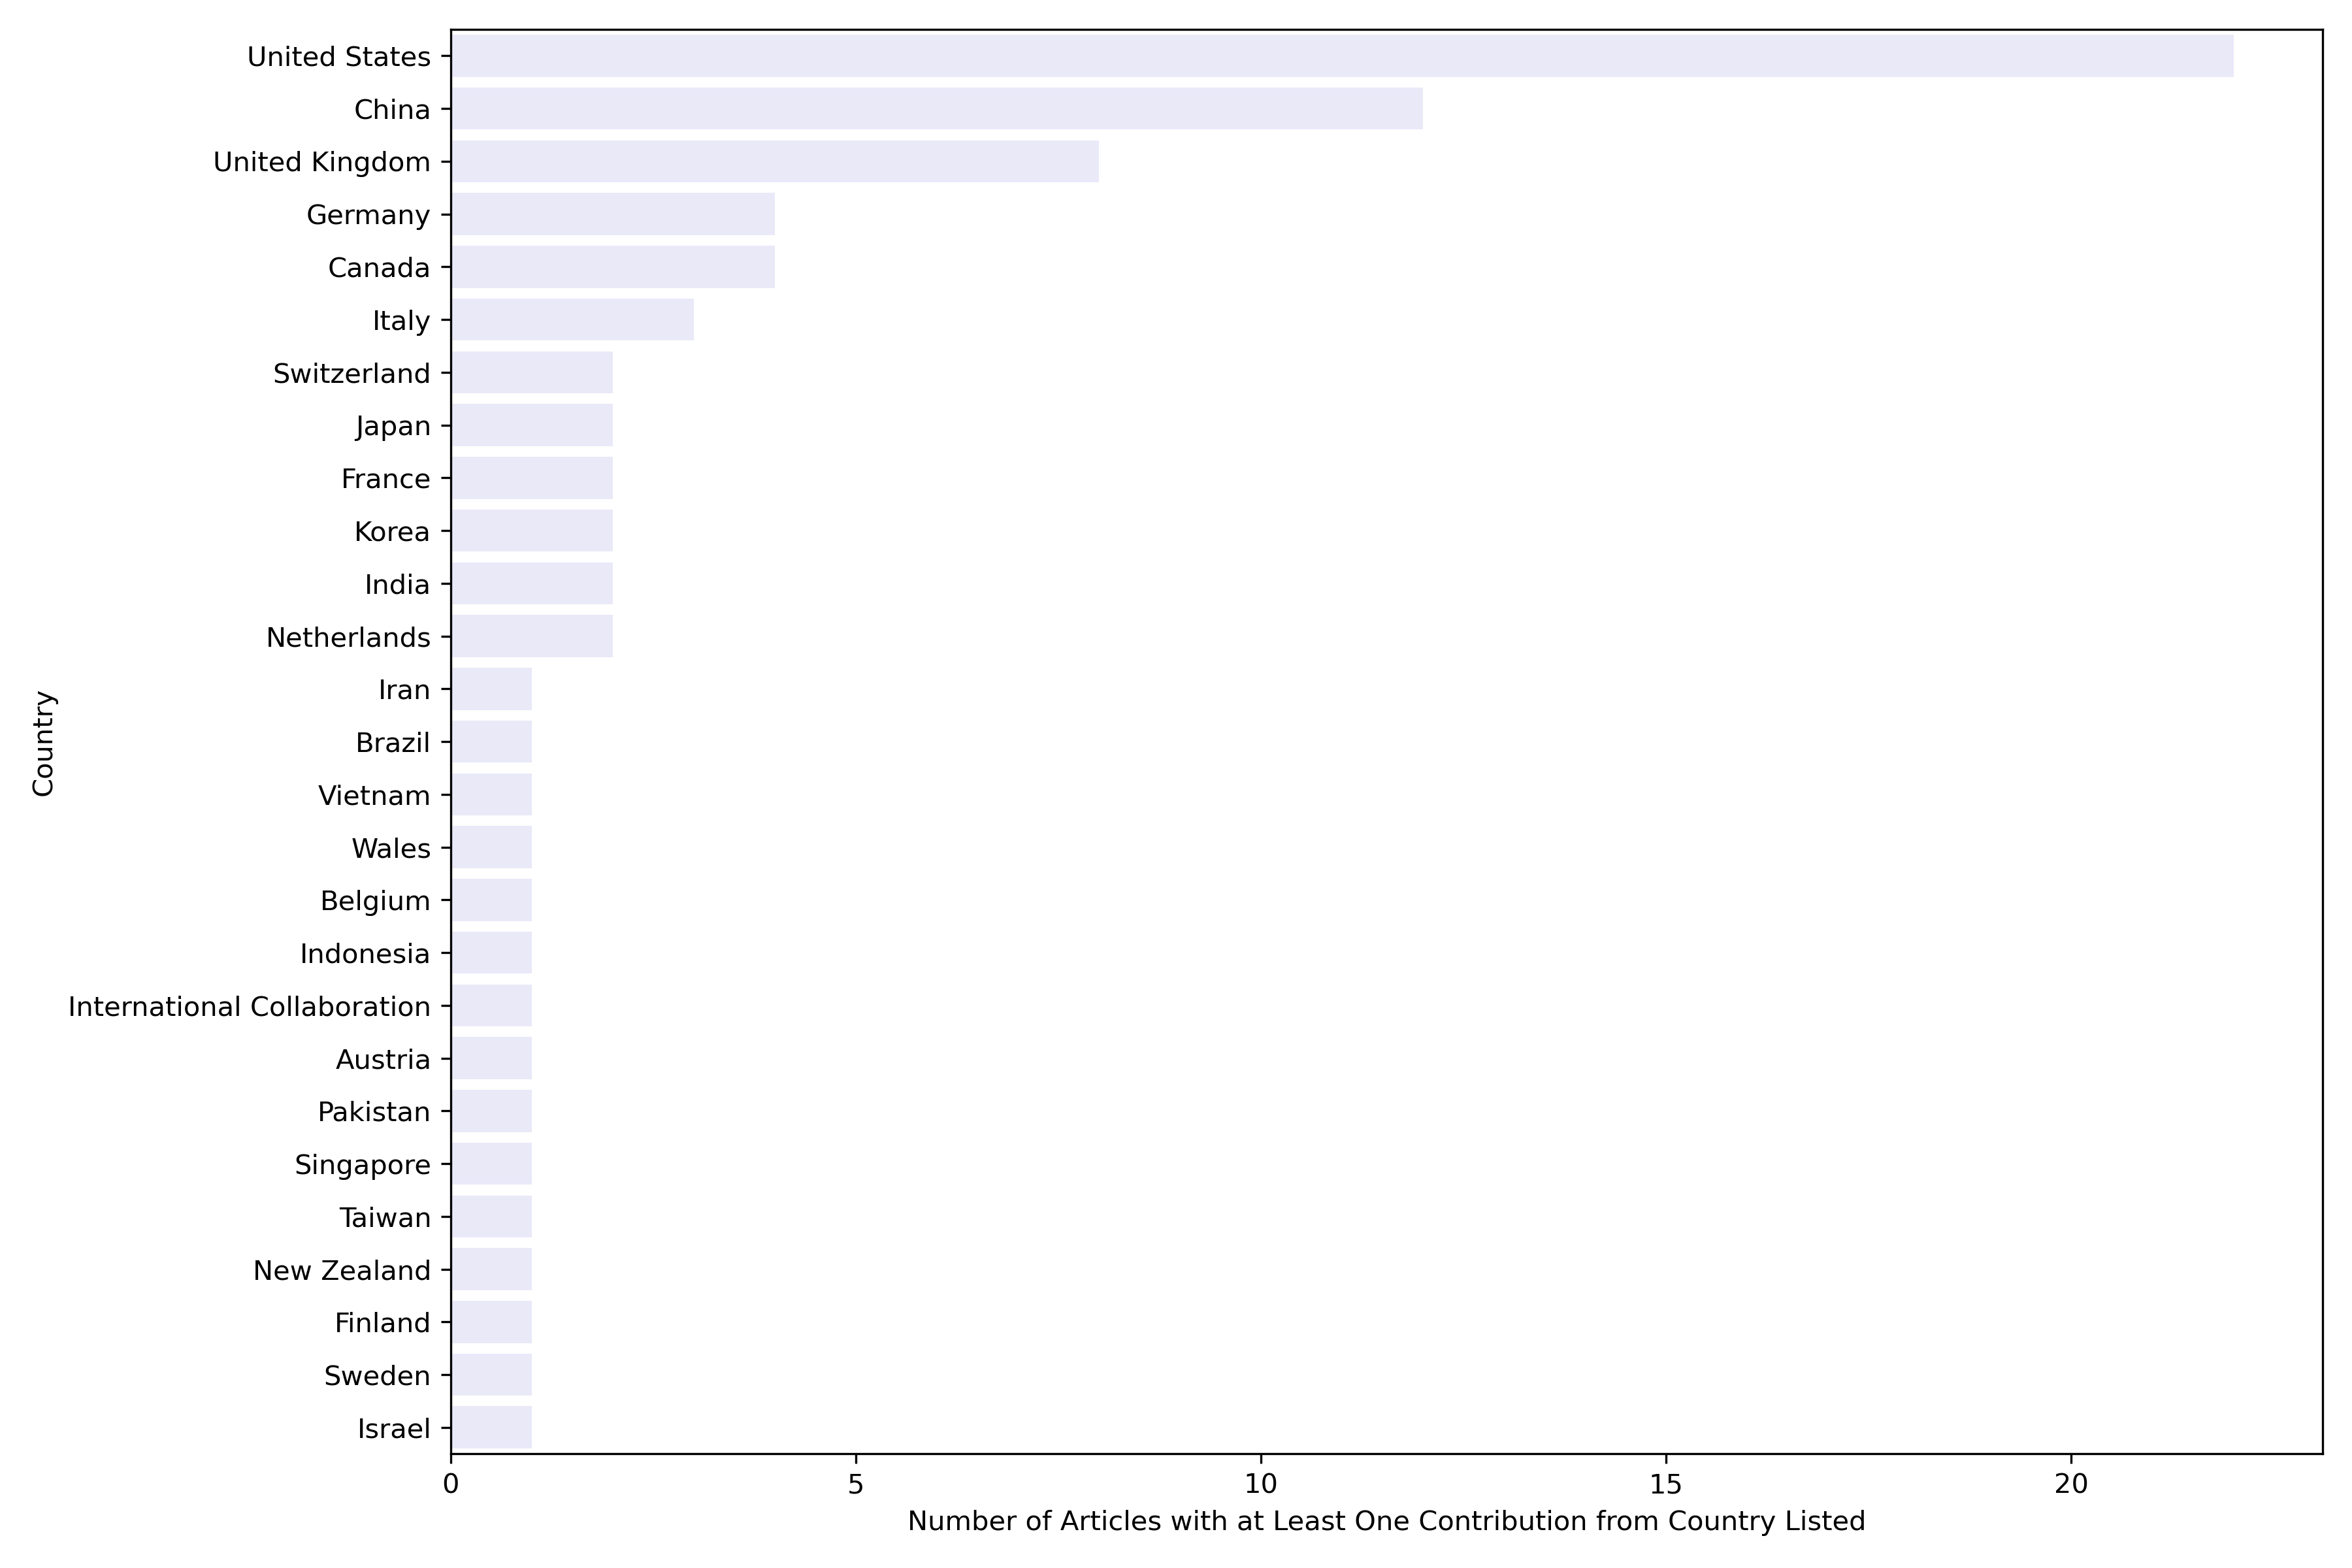
\includegraphics[width=\textwidth]{figs/countries.png}
    \caption{Number of articles in final subset who have at least one author from the listed country. ``International Collaboration'' denotes too many countries to list.}
    \label{fig:country}
\end{figure}

\begin{figure}[ht!]
    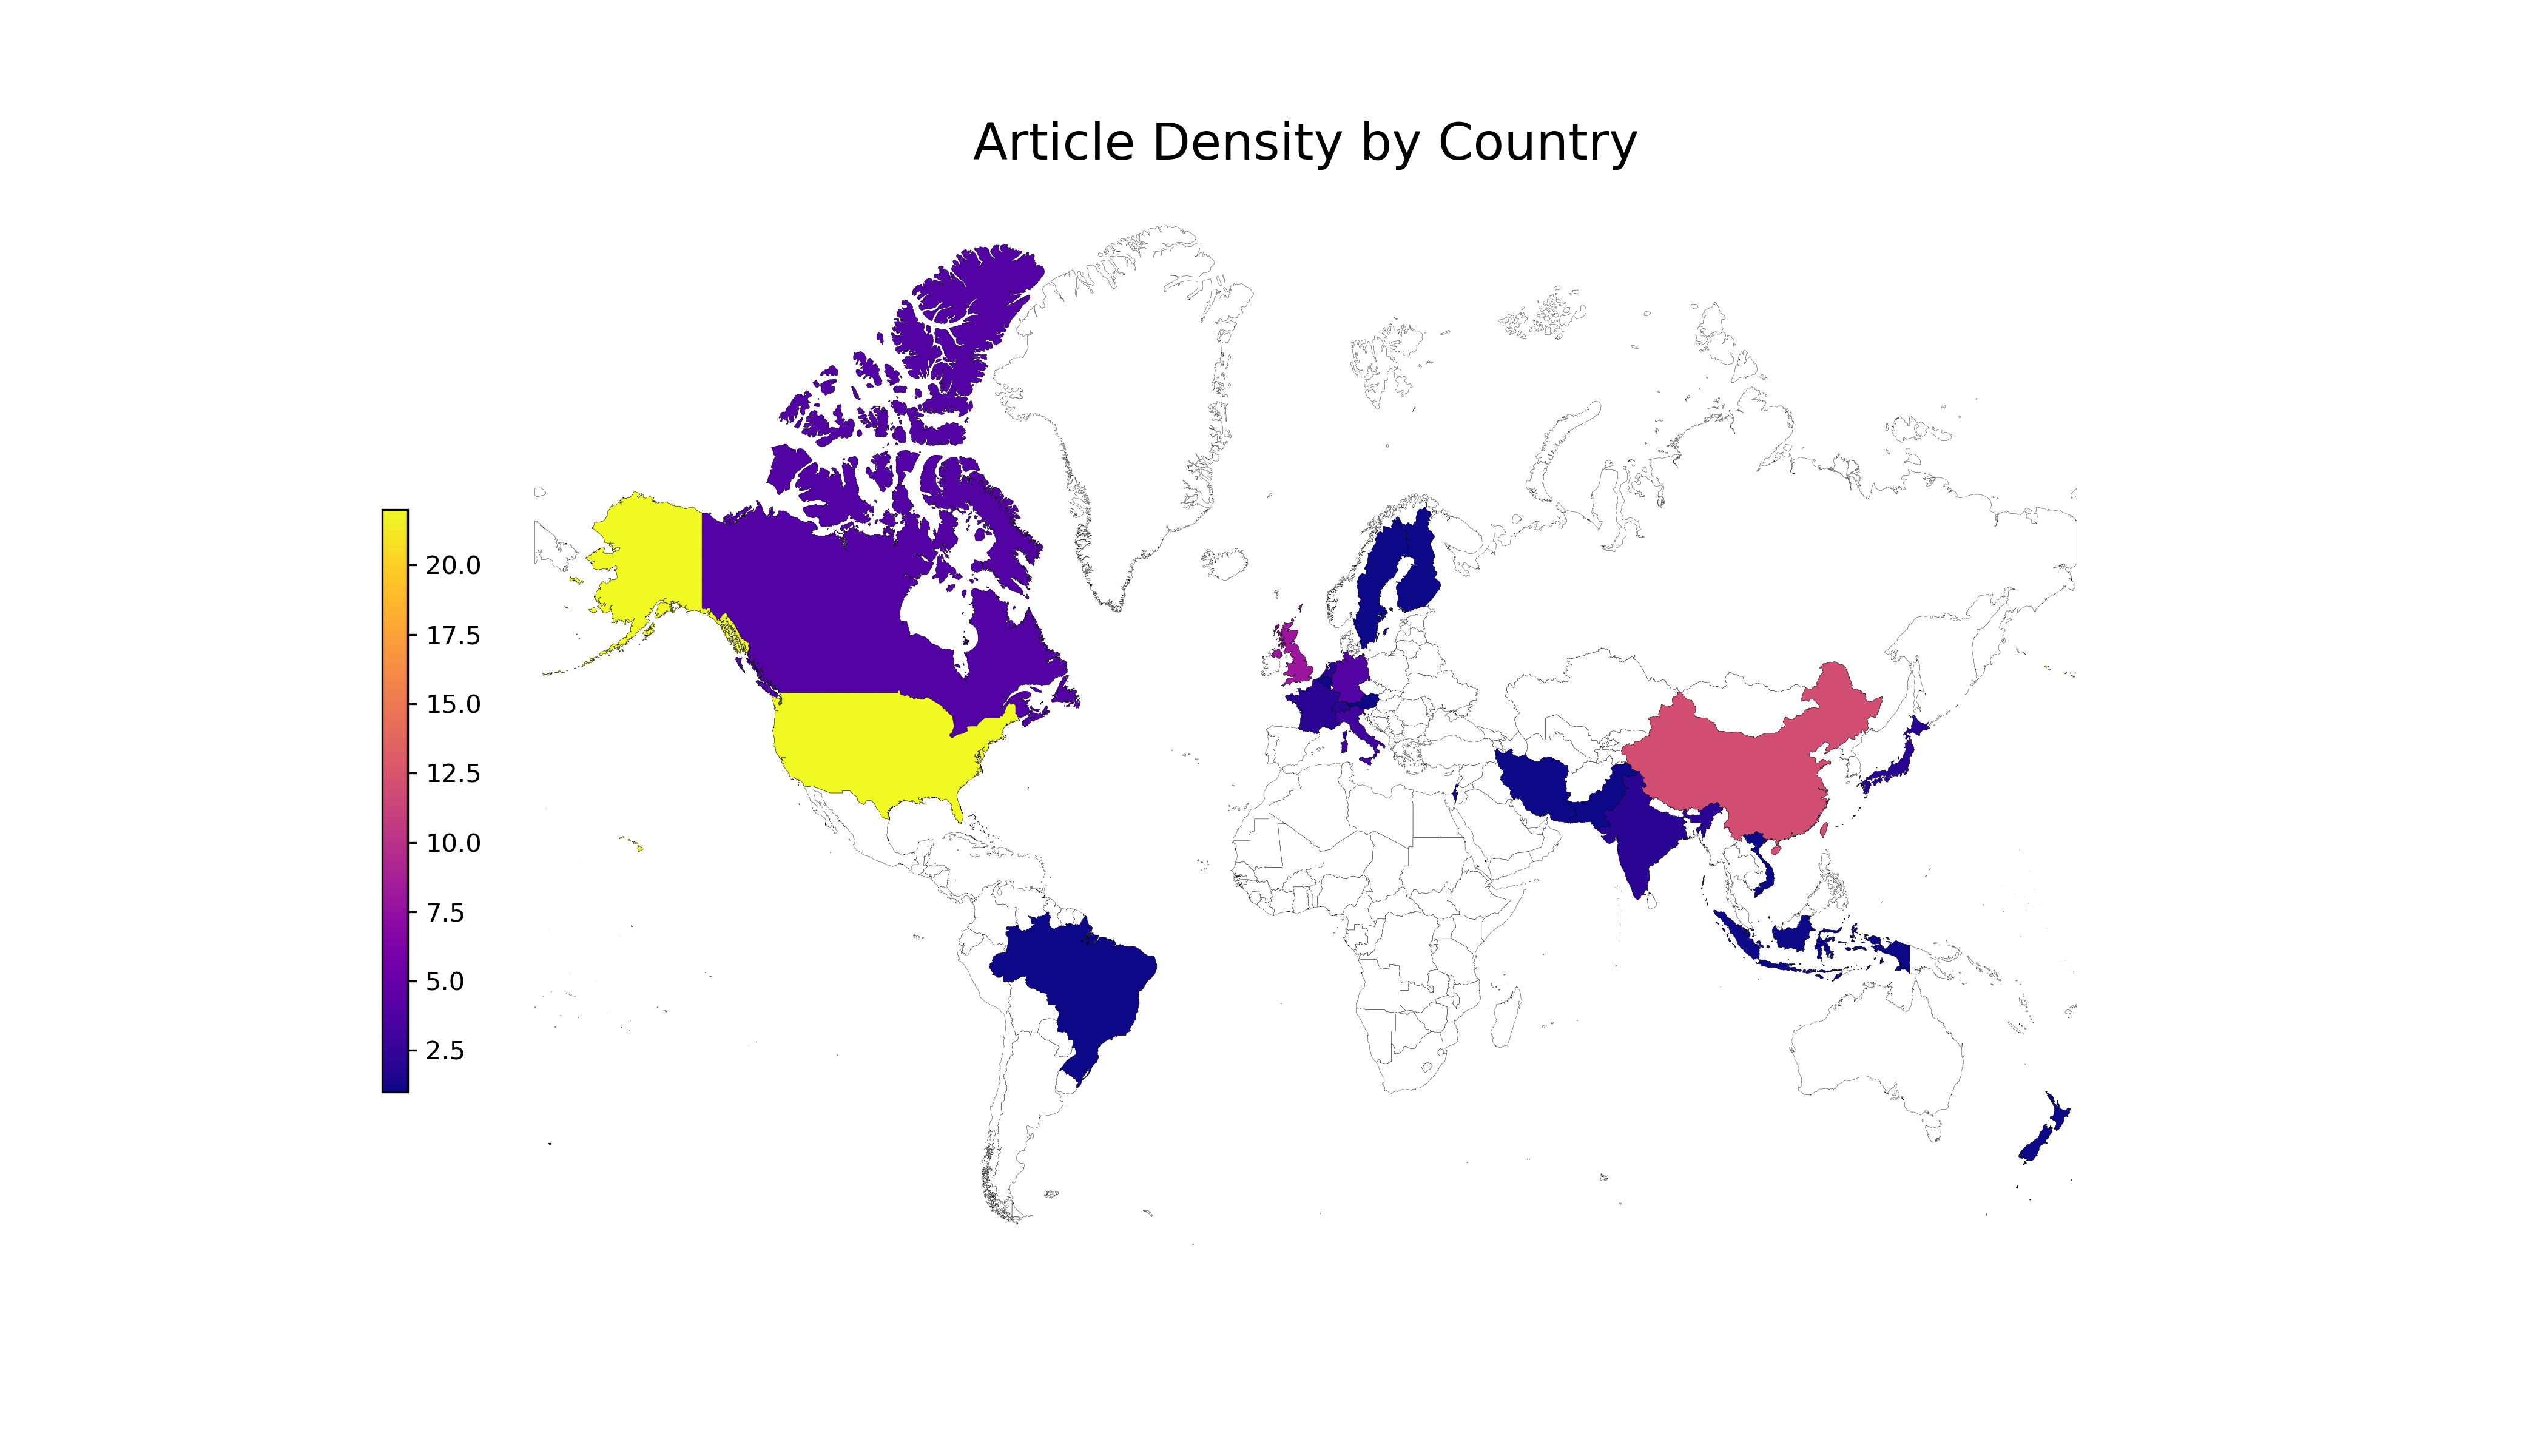
\includegraphics[width=\textwidth]{figs/countries_map.png}
    \caption{Number of articles in final subset who have at least one author from the listed country. ``International Collaboration'' article is excluded from this figure, see attached database for details.}
    \label{fig:country_map}
\end{figure}

Finally, Table \ref{tab:industry_distribution} shows the distribution of articles by industry for the final subset.

\begin{table}[ht!]
    \centering
    \begin{tabular}{lr}
        \toprule
        Industry & Percent of Final Subset of Articles \\
        \midrule
        Medical & 59.72\% \\
        Autonomous Vehicles & 18.06\%\\
        Nuclear & 9.72\% \\
        Aviation & 8.33\% \\
        Ethics & 2.78\% \\
        Manufacturing & 1.39\% \\
        \bottomrule
    \end{tabular}
    \caption{Final article subset distribution by industry. \textcolor{red}{Should I keep or remove the percent signs here?}}
    \label{tab:industry_distribution}
\end{table}

\section{Qualitative Results and Discussion}
The quantitative data provided in Section \ref{sec:quantitative_results} only  tell a fraction of the story. During the data extraction process, we took analysis notes and highlighted key findings from each study in the final subset. To best introduce these findings, we will first discuss each of the major industries identified in our study, highlighting key takeaways from the individual industries and some papers that brought especially unique points to our attention. Then, we will examine the similarities and differences between the various industries to determine what AI features and findings were universally beneficial, and which industries have specific challenges and demands.

\subsection{Medical}
\label{sec:medical}
Medical papers comprised nearly 60\% of our final subset of articles (see Table \ref{tab:industry_distribution}). As the largest industry in article numbers from both the query results and the final subset analysis, the medical industry has a lot to offer in terms of experience using AI systems and highly sensitive usage demands. AI in this industry generally has greater decision-making times and interfaces usually with highly skilled professional (like doctors), but can also interact directly with patients. Due to its size and variety, we break down this group of papers into smaller categories, as described in the following subsections. 


\subsubsection{Pharmacology}
Eight out of the 43 papers categorized as medical considered applications related to the prescribing and dispensing of medication--- we labeled these papers under ``pharmacology.'' Only two of these papers considered regulation, while three considered model explainability. Interestingly, two of the papers that did consider explainability evaluated large language models (LLMs), which are widely considered the most opaque. 

The aforementioned articles \cite{ongLargeLanguageModel2025} and \cite{chaseEvaluationLargeLanguage2025} both evaluate LLMs as medication safety-focused clinical decision support systems (CDSS), including prescription errors and drug-drug interactions. Both \cite{ongLargeLanguageModel2025} and \cite{chaseEvaluationLargeLanguage2025} evaluated variants of Gemini, ChatGPT, and Claude. Ong et al. evaluate the success rate of identifying ``drug-related problems'' (DRPs) in three scenarios: pharmacist alone, pharmacist with AI-assistance (co-pilot mode), and AI alone and found co-pilot mode to yield the highest success of DRP identification \cite{ongLargeLanguageModel2025}. Chase et al. do not consider AI-pharmacist cooperation, and instead evaluate the LLM independently, still substantiating the finding that the LLMs perform suboptimally alone. They found the LLMs to make potentially harmful clinical recommendations up to 15.4\% of the time (ChatGPT) \cite{chaseEvaluationLargeLanguage2025}. Chase et al. also raise concerns for the less overtly dangerous but still problematic scenario of suboptimal recommendations, such as flagging non-clinically relevant drug interactions, which can lead to alert fatigue over time \cite{chaseEvaluationLargeLanguage2025}. These reports highlight the importance of studying not only the pure accuracy of AI systems, but how they interface with and \hl{cooperate} with their users.
\textcolor{red}{Not sure if this is the right word, looking for ``co-thinking'' but collaborate and cooperate both sound like they need to be person-person.}

In response to their findings, Chase et al. directly call for both external validation and benchmarking of medical AI against existing standards \textit{and} model explainability techniques to address the black-box nature of LLMs before they are implemented into clinical practice \cite{chaseEvaluationLargeLanguage2025}. Ong et al. state that the LLMs tested (ChatGPT, Gemini, and Claude) offer something that many ``explainable AI tools'' cannot--- ``conversational interfaces [that] allow clinicians to ask questions and receive context-specific explanations in plain language'' \cite{ongLargeLanguageModel2025}. While the conversational nature of chatbots may seem like a more approachable ``explanation,'' this logic can be dangerous as reasoning provided by a chatbot is \textit{not} a true explanation and does not indicate \textit{any} amount of model reliability, accuracy, or trustworthiness. We caution that this reasoning may lead to complacency and instead urge practitioners, regulators, and developers to consider genuine explainability and validation methods when applying these tools in practice. Explainability, in particular, can help the ultimate decision-maker (the pharmacist or prescriber) rationalize the CDSS recommendation, giving them grounds to dismiss or accept it with cause.

The remaining articles in the pharmacology subcategory use either classical ML techniques (decision trees and gradient boosting) (\cite{kieuDevelopmentValidationMachine2024}, \cite{buckerArtificialIntelligenceAssist2024}, \cite{cornyMachineLearningbasedClinical2020}), association rule learning (\cite{chenAbilityMachinelearningBased2024}), and CDSS built-in systems (\cite{nimriInsulinDoseOptimization2020}, \cite{liuDiscrepancyPerceptionsAcceptance2023}). Of these, Kieu et al. considered decision trees explicitly for their inherent interpretability \cite{kieuDevelopmentValidationMachine2024}. From a deployment perspective, Liu et al. is a qualitative study of pharmacist interviews on trusting CDSS recommendations, which found that after consulting a CDSS, 78\% of pharmacists did not adjust their dosing regimens due to ``distrust and lack of understanding of the justification of the CDSS recommendations'' among other concerns, despite a ``generally positive attitude toward CDSS'' \cite{liuDiscrepancyPerceptionsAcceptance2023}. This supports claims made by papers throughout this report that model trust is paramount to implementation and that this trust is often coupled with explainability or ``justification.'' Even if a co-piloted pharmacist-AI approach yields the safest medication prescription and dispensing, without pharmacist trust in the partnership, the accuracy improvements are moot. 

\subsubsection{Imaging and Diagnostics}
Eight of the 43 papers evaluated in this section evaluated using AI for diagnostic and/or imaging techniques. Of these papers, specific AI techniques included convolutional neural networks (CNNs) for classification of glaucoma \cite{vieiraExploringTransparencyComparative2025}, LLMs for emergency medical advice \cite{yauAccuracyProspectiveAssessments2024}, generative adversarial networks (GANs) and other methods for skin lesion classification \cite{mettaAdvancingDermatologicalDiagnostics2024}, decision trees for cervical spine injury diagnosis \cite{bertsimasPredictionCervicalSpine2019}, and CNNs for stroke onset time prediction \cite{akayDeepLearningAnalysis2023}. Of the remaining three papers, two included perspective papers from both leaders in emergency medicine on incorporating AI into their practices \cite{taylorLeveragingArtificialIntelligence2025} and patients on AI being used to evaluate their prostate cancer screening MRI results \cite{fransenPatientPerspectivesUse2025}. These perspective studies will be evaluated with the other qualitative pieces in Subsection \ref{sec:qualitative}. The last paper in this category discusses AI in radiology more broadly and in light of the increased rate of AI use in published radiology papers, offers methods to increase generalizability by overcoming overfitting and underspecification \cite{echeGeneralizabilityDeploymentArtificial2021}. 

Of the articles considered in this subsection, four of them consider regulation and five of them consider explainability. Of those that consider both, Vieira et al., who use various explainable AI techniques to support glaucoma diagnosis, presents one of the most explainability-forward papers in this review \cite{vieiraExploringTransparencyComparative2025}. The authors use retinography images on CNNs coupled with CAM, GradCAM, LIME, SHAP, vanilla gradients, SmoothGrad, and SCIM to evaluate the quality of the different explainability methods for a high risk clinical application (blindness) \cite{vieiraExploringTransparencyComparative2025}. The authors partnered with an ophthalmology specialist while conducting their analysis to evaluate the utility of the various explanations generated by the methods in their study. They found CAM-based methods to be the most effective way to reliably support diagnosis via its clear identification of clinically relevant regions and intuitive visual interpretation \cite{vieiraExploringTransparencyComparative2025}. 

Vieira et al. present a forward-thinking study in their work, anticipating and acting on the needs of clinicians to understand model results by evaluating a variety of explainability methods. While inherently interpretable models, like decision trees, can offer a clearer, more straightforward understanding of model logic, simpler models are not always an option. Especially in the imaging and diagnostic realm, the necessary data types (image-based) may not lend themselves well to the limited number of inherently interpretable ML methods available. In situations like these, to capitalize on more advanced model performance, we must develop ad-hoc explainability methods to understand the results in a way that makes them reliable and comprehensible for clinicians when the stakes are high. Vieira et al. do just that, and it is likely that future work will emulate them in other highly sensitive domains as experts drive demand for rationalized AI recommendations.

\subsubsection{Radiation and Other Treatment}
Nine of the 43 papers reviewed in this section evaluate the use of AI to design and carry out treatment plans with six of those nine specifically considering radiation treatment. The number of radiation treatment studies that employ AI alone represents the perceived utility of AI at improving highly sensitive treatment outcomes, as this subset of papers discusses the precision required in radiation treatment. Of all nine papers considered in this section, six of them considered some aspect of explainability, but only one of them considered regulation. The paper that considered regulation was an insulin dose optimization method for Type I diabetes already deployed in the AI-DSS DreaMed Diabetes Pro. This paper considered oversight by the U.S. FDA but did not consider any explainability \cite{nimriInsulinDoseOptimization2020}. Of the radiation treatment papers considered, nearly all employed classical ML methods, including decision trees, random forests, support vector machines, and gradient boosting. Only one paper (\cite{chenEvaluationAutomatedClinical2024})considered UNets, a type of CNN, exclusively, and another paper considered neural networks in addition to classical methods (\cite{chamseddinePredictiveModelingSurvival2022}). Four (\cite{alizade-harakiyanDecisionTreebasedMachine2025}, \cite{fleuryStereotacticRadiationTherapy2025}, \cite{chamseddinePredictiveModelingSurvival2022}, \cite{braunMachineLearninggeneratedDecision2022}) of these six papers either conducted feature importance studies on these classical methods or rationalized using an inherently interpretable model for explainability purposes. Additionally, Komorowski et al. used reinforcement learning as the primary learning method for intensive sepsis care, but still used random forests to determine clinically interpretable reasoning (importance of model parameters) \cite{komorowskiArtificialIntelligenceClinician2018}. The majority of these studies indicate a preference towards simpler, more comprehensible models, and an even greater majority employ explainability for highly sensitive treatment methods.

Most of these papers considered AI to find some threshold dose that is sufficient for treatment success while minimizing harm and secondary radiation side effects to the patient. One of the papers that did not consider explainability outright, did perform an uncertainty analysis on their UNet model for dose prediction to treat prostate cancer, which still highlights a need to establish model trust \cite{chenEvaluationAutomatedClinical2024}. Overall, the trend in treatment papers towards explainable AI-decision-support methods supports what we saw in pharmacology-- that experts need rationalized recommendations before implementation. Further, the one paper \cite{nimriInsulinDoseOptimization2020} that interfaced directly with patients was validated through clinical studies and regulated by the FDA, because it was not subject to expert oversight.

\subsubsection{Legal and Regulatory}

\textcolor{cyan}{@Riley, please review this section and add details where you see fit! You can recommend cutting information using the \st{strike through} command \\st\{text here\}}

Eight of the 43 articles considered under the ``medical'' umbrella directly concerned legal and regulatory factors. Unlike other subsets, these papers generally do not evaluate a specific type of AI. Instead, they describe the ethics, liability, and regulatory considerations that govern these technologies in sensitive domains. Of the eight, five legal/regulatory papers consider explainability in their discussions. In terms of governing bodies concerned, three papers are from E.U. member states, two are from the U.S., two are from the United Kingdom, and one is from Canada. 

Of the articles we considered in this subsection, we identified alignment on the theme of trust. 

% Trust can be broken up into three parts: truth claims, commitment, competence
Jones et al. base their arguments explicitly following Onora O'Neil's previously established trust framework \cite{jonesArtificialIntelligenceClinical2023}. This framework has two major tenets. The first is that trust and trustworthiness are two distinct concepts that ought not to be conflated. Trust is only dangerous when misplaced into an untrustworthy entity and further that \textit{``only beings with agency are truly capable of being trusted''} \cite{jonesArtificialIntelligenceClinical2023}. Oftentimes, we can define the individuals issuing trust and those assessing trustworthiness as separate cases. In the industries considered in this review, when the public is a direct user of an AI-based decision-making system, we must assume they do not have the expertise to assess trustworthiness of that system. Therefore, these individuals must trust the judgment of some other trustworthiness assessor. For safety-critical industries, as an example, this assessor could be the regulator. In other words, the public places their trust in the regulator, not in the AI itself. 

Alternatively, if the direct user of an AI-based decision-making system \textit{does} have the expertise to assess that system's trustworthiness (such as a medical professional), then they can decide on a case-by-case basis when they are willing to accept its recommendations, and they can serve as a barrier to the less knowledgeable public. In this case, the public places their trust in the experienced professional, not in the AI itself. 

Unfortunately, the ``agency'' argument can be complicated for AI with varying levels of autonomy, and in reality, the two cases outlined above may not be so clear-cut. Trust may fall reasonably back on model developers, users, procurers, etc. \cite{jonesArtificialIntelligenceClinical2023}. This distinction could prove critical when it comes to determining liability issues with the implementation of AI systems, a topic considered by many papers in this subgroup. Following O'Neil's logic, if a system possesses no agency, it cannot be trusted, and therefore that trust cannot be violated. The liability question then becomes: \textit{Who is responsible for the consequence of this system?} This is the debate of many legal experts and should be considered by all participants in an AI system, especially as laws and regulations surrounding these technologies change. As a potential solution, Lagiola et al. and Labkoff et al. suggest that unique regulations should correspond to classes of AI automation levels to define the shared the level of responsibility and liability between the AI system and the individuals involved it its use \cite{lagioiaStrangeCaseDr2020}, \cite{labkoffResponsibleFutureRecommendations2024}. 

The current licensing system in the U.S. is more vague than that and leaves many of the aforementioned questions up to the courts. Instances where AI-assisted decision systems are used by a skilled professional are less regulated and instead rely on their expert judgment (and malpractice insurance). \textcolor{red}{Too cheeky?} Medical AI systems that interface directly with the public, on the other hand, mainly qualify as medical devices, and can be regulated as such in the U.S. 

Briefly, if you design a nonexempt medical device (excludes items like Band-Aids and gauze), you have three main pathways for licensing through the FDA: Premarket Approval (PMA), 510(k), and De Novo \cite{gerkeNewCaseLaw2025}. The first, PMA, is the most rigorous and typically requires clinical trials to demonstrate ``reasonable safety and effectiveness,'' whereas the 510(k) pathway only requires demonstrating ``equivalence'' to a predicate device \cite{gerkeNewCaseLaw2025}. The latter is faster and designed for lower risk devices (Class I and II), but offers less litigation protection from state tort claims. Finally, De Novo offers a bit of a hybrid pathway that offers neither all the protections of PMA nor all the speed of 510(k) and yields highly uncertain outcomes as few courts have ruled on De Novo cases to date \cite{gerkeNewCaseLaw2025}. De Novo devices are considered novel but lower risk than PMA devices, so some clinical data may be provided during licensing, but the safety and efficacy assessment is less rigorous than PMA. 

Amidst the legal nuance, the uncertainty of the De Novo pathway is important when we consider medical AI because, according to Gerke et al., ``Manufacturers of AI/ML-enabled devices successfully used the De Novo pathway about three times more often than did most device manufacturers,'' demonstrating proclivity for these companies to opt for uncertainty \cite{gerkeNewCaseLaw2025}. This may concern the public as they rely on the FDA's trustworthiness assessment for these (and non-AI) devices-- is this level of review sufficient to ensure patient safety? A more thorough approach may include rigorous validation techniques and/or a unique licensing pathway for a unique set of technologies. 

% BIAS
One ethical concern of AI-based medical devices, emphasized by McCradden et al., Kiseleva et al., DeMicco et al., and many others is the impact of bias in AI systems \cite{mccraddenPatientSafetyQuality2020}, \cite{kiselevaAreYouAIS2021}. Aside from ethical misgivings, biased AI systems may have legal implications as well, at least in medical contexts. Gerke et al. describe that when licensing a medical device, you license it as-is. It is possible, however, that ``continuously learning'' or even discretely retraining an AI system will worsen efficacy for certain patient groups \cite{gerkeNewCaseLaw2025}. Shah et al. extend this concern to broader changes post-market release \cite{shahRegulatoryLegalConsiderations2025}. Failure to warn users of these changes could leave manufacturers liable, even if their original model was protected. Changing efficacy across patients groups, however, may be difficult to assess without formal validation techniques. Thus, aside from being ethically valuable to consistently validate and evaluate your model for bias, we also find legal motive to embed this into system design.

When validation methods are not perfectly accurate, explainability methods offer a second layer of protection to the patient, doctor, and AI manufacturer. As explained by DiMicco et al., ``AI systems should be developed to enable humans to understand their actions and the underlying logic in order to increase transparency and minimise the risk of bias or error'' \cite{demiccoRoboticsAIHealthcare2024}. Some jurisdictions have already begun to require aspects of explainability, such as in the European General Data Protection Regulation (GDPR) Articles 13 and 14, which require ``meaingful information about the logic involved, as well as the significance and the envisaged consequences of such processing'' when decision-making is automated \cite{lagioiaStrangeCaseDr2020}.

% Over Trusting
The second tenet of O'Neil's argument, described in Jones et al. are the three constituents of trust: trust in truth claims, trust in commitment, and trust in competence \cite{jonesArtificialIntelligenceClinical2023}. The first is an empirical evaluation, \textit{is this entity likely to give me a factually correct answer?}, whereas the second two are normative, \textit{is this entity likely to follow through on their promises?}, and \textit{is this entity likely to execute the promised action successfully?}. As developers, we typically focus on the empirical arm of these, and this is evident on the way we evaluate AI systems: \textit{given 1,000 scenarios, how often will my system predict the correct answer?} We have a plethora of ways to describe the mathematical nuances of this question, $R^2$, $F1$, mean absolute error, etc., yet we seldom consider the other two thirds of how people think about trust when we set out to develop a ``trustworthy system.'' 

The tendency for individuals to place undue trust in these systems by focusing on the normative elements is evident. After considering the perspective of clinicians incorporating AI into their practice and the empirical trust issues they experience, Jones et al. also consider how patients feel about their doctors using AI. They summarize several studies that asked hypothetical patients how they would view various outcomes when their doctors did or did not use AI systems. Overwhelmingly, they found that patients at worst had no difference of opinion when AI is used, and at best, view their doctors' decisions more favorably, even if the outcome is still unfavorable, showing that AI may serve as a ``protective shield'' for clinicians \cite{jonesArtificialIntelligenceClinical2023}. 

There are, of course, some caveats to this: the studies were hypothetical and generally assumed that the AI in question had a known superior diagnostic accuracy than the doctor \cite{jonesArtificialIntelligenceClinical2023}. Jones et al. conclude that patient favorability towards using AI stems from higher normative trust in two ways. One, that AI is both reliable (machines tend to be more predictable than humans) and two, that AI is competent (on the basis of mass amounts of training data) \cite{jonesArtificialIntelligenceClinical2023}. They warn that this trust may be misplaced. Both the readiness of patients to (blindly) trust AI and the clinician's concerns about its empirical accuracy further support the case for co-piloted AI-clinician systems and raises red flags for autonomous AI healthcare providers. 

Despite public overconfidence in AI system, domain experts tend in the opposite direction. In a trial run of AI-assistance at the U.S. FDA to analyze causality in individual case safety reports (ICSRs), reviewers rejected the AI's analysis in most cases because ``...the approach did not offer sufficient explanation or flexibility to accommodate information external to the ICSR (e.g., reviewer's knowledge)'' \cite{ballTrustVerifyLessons2024}. Further, ``Because of the lack of trust in the software tools, any efficiency gains... were not perceived as making it easier for the safety reviewers...'' \cite{ballTrustVerifyLessons2024}. This highlights a case where domain experts not only question the AI's truth claims, but also its competence given a lack of sufficient data. The critical feature of this scenario is \textit{the expertise of the reviewer}. A less knowledgeable individual may more readily accept the claims of an untrustworthy system, simply because they did not know better. This underscores the importance of ``human-in-the-loop'' systems, as described by \cite{jonesArtificialIntelligenceClinical2023}, and the urgent need to maintain the proficiency of subject-matter experts. 

Despite findings that experts remain dubious of unexplainable AI, developers and regulators should still consider ways to counter ``automation bias'' \cite{jonesArtificialIntelligenceClinical2023}. In other words, how can we prevent domain experts from doubting their own judgment when AI suggests a (potentially wrong) alternative? \textit{How can we encourage them to ``trust their gut?''} Holding professionals accountable for decisions in their fields may encourage this. Even still, how can we ensure that experts are protected when they rely on their own professional expertise? Explainability measures may mitigate automation bias by allowing practitioners to critically analyze the reasoning of the AI, creating a situation more similar to a collegial disagreement. Still, future work should consider implementing guardrails in software design for these known shortcomings of AI-assisted decision-making systems, and \hl{regulation should protect domain experts' right to independent thinking.} \textcolor{red}{Too strong?}


\subsubsection{Qualitative Analyses and Roadmaps}
\label{sec:qualitative}
% Include Taylor 2025 (EM perspective) and Fransen 2025 (prostate cancer perspective) here instead of in diagnostics
The final medical category consisted of five qualitative papers. This included two from diagnostics (\cite{taylorLeveragingArtificialIntelligence2025} and \cite{fransenPatientPerspectivesUse2025}). Of these five, one focused directly on healthcare professionals' perspectives (\cite{nouisEvaluatingAccountabilityTransparency2025}) while another focused directly on patient perspectives (\cite{fransenPatientPerspectivesUse2025}). The remaining three make broad recommendations on what AI in healthcare ought to look like, all of which included addressing risk of bias, validation, regulation, and explainability as key issues \cite{labkoffResponsibleFutureRecommendations2024}, \cite{fuchsLindberghsCockpitPredictive2025}, \cite{taylorLeveragingArtificialIntelligence2025}. As a protective mechanism, Labkoff et al. propose an CDSS-incident reporting platform, so that we can continuously learn from mistakes made by these systems \cite{labkoffResponsibleFutureRecommendations2024}. Additionally, they recommend a standardized way of informing clinicians what each tool can be used for and what its limitations are, much like a ``nutrition label'' for technology \cite{labkoffResponsibleFutureRecommendations2024}. In a similar vein, Taylor et al. emphasize the importance of mitigating bias through model ``validation across institutional datasets,'' highlighting a need for cross-institutional collaboration \cite{taylorLeveragingArtificialIntelligence2025}. Unfortunately, sensitive applications like healthcare also come with sensitive data. This is a challenge we can expect across sensitive domains that may be addressed with organizational efforts or federal guidance. 

Finally, our two interview-based perspective papers, Nouis et al., which focused on professional perspectives, and Fransen et al., which focused on patient perspectives offered insight from both sides of medical practice. Nouis et al. found that the professionals they interviewed, including doctors, nurses, staff scientists, and administrators all similarly raised concerns about the reliability of ``black box models that lack clear rationale or interpretability'' and risk of bias of these systems, especially because they felt ultimately liable \cite{nouisEvaluatingAccountabilityTransparency2025}. The patients interviewed in Fransen et al. were admittedly a nonrepresentative sample set of mostly highly educated, white men with prostate cancer \cite{fransenPatientPerspectivesUse2025}. These individuals showed a clear preference for using AI versus not to aid radiologist's judgment of their cancer imaging, but only 15\% preferred a completely autonomous AI system with no radiologist oversight \cite{fransenPatientPerspectivesUse2025}. Fransen et al. acknowledge the limitations in their study by referencing a different outcome found by an older study on women's acceptance of AI in mammogram interpretation that found a notably lower level of acceptance \cite{fransenPatientPerspectivesUse2025}. This difference could be attributed to a variety of factors other than gender, including the year of publication (2025 for Fransen et al. and 2021 for the mammogram study), but it highlights the importance of not just evaluating bias within the model but also understanding how accepting individuals may be of them.

\subsection{Autonomous Vehicles}
Autonomous vehicles comprised just over 18\% of our final subset of articles, our second-largest category. These papers ranged from focusing directly on ethics (\cite{eggertAutonomisedHarming2025}, \cite{guensbergAutomatedVehiclesDilution2022}, \cite{geisslingerEthicalTrajectoryPlanning2023}, \cite{bertheauEventrelatedPotentialsReveal2025}), to validation (\cite{yangPredictionFailureRiskaware2023}, \cite{jiAcceleratedTestingEvaluation2025}), explanations (\cite{fengNLEDMNaturallanguageExplanations2023}, \cite{kanekoPredictingTrustDynamics2025}), legal implications (\cite{maLegalDecisionmakingHighway2023}, \cite{tianHowShouldAutonomous2025}), and pure accident avoidance (\cite{goodallComparisonAutomatedVehicle2021}, \cite{luPhysicsinformedAttentionModel2025}). Broadly looking at the subcategories alone highlights some unique distinctions from the other industries in this review. First, the overwhelming number of ethics-focused papers. Unlike in medical contexts, autonomous vehicles often face two-body ethical dilemmas-- who should be spared in an unavoidable collision scenario? Further, an increased need for validation and regulation is clear. 

Autonomous vehicles, as their name implies, do not enjoy the protections of ``human-in-the-loop'' systems, which is what most medical AI operates under. Nor do the users of these AI-driven system reap the benefit of a certified expert reviewing each and every decision. Instead of the AI offering a suggestion and an experienced professional using their expertise to decide whether to take it, autonomous vehicles make decisions nearly continuously and rely on human intervention \textit{only} if something goes awry. This removes a barrier of protection against unreliable systems, making liability issues more complicated, especially when defining what ``human intervention'' looks like. How can you expect someone to intervene on a system that was designed to relieve their attention span? Tian et al. approach this argument by promoting proactive insurance involvement and liability rules that encourage manufacturers to invest in safety \cite{tianHowShouldAutonomous2025}. Simply, Tian et al. explain this in the context of the Hand Formula-- if the burden (of safety innovation) is less costly than the probability (of an accident) times the loss (of that accident), it is negligent for the manufacturer \textit{not} to take that safety precaution \cite{tianHowShouldAutonomous2025}.

To make the safety designation even more challenging, although many of the AI systems evaluated in this paper are ``narrow AI,'' meaning they are trained for a specific task (the opposite of general AI), autonomous vehicles face a wide variety of scenarios, and can struggle to learn edge cases that have severe consequences (as seen in \cite{yangPredictionFailureRiskaware2023}). This combined with a lack of general oversight points to a major need for validation methods that can serve as the basis of verifying the safety of these systems to the public. This is perhaps why we see the most validation studies in this subcategory-- two (\cite{yangPredictionFailureRiskaware2023}, \cite{jiAcceleratedTestingEvaluation2025}), versus one for aviation (\cite{mossBayesianSafetyValidation2024}), and none for any other category. 

Generally, we denote validation and explanation as distinct but similarly useful practices for AI-supported decision-making. In the context of autonomous vehicles, however, the latter is less effective. While explanations can be helpful in understanding the rationale of an autonomous vehicle's decision-making, they are less useful than CDSS explanations because the window of time between an autonomous vehicle's data acquisition, modeling calculation, and decision is much shorter. In other words, one would probably hope that a doctor takes more time to decide a patient's stroke treatment plan than they take to change lanes on their way to work. The same time restriction on those decision-making scenarios applies for autonomous vehicles, so model explanations are not particularly useful for human intervention. 

Counterintuitively then, two papers in this category focus \textit{primarily} on developing model explanations (\cite{fengNLEDMNaturallanguageExplanations2023}, \cite{kanekoPredictingTrustDynamics2025}). In these reports, explanations play other roles than rationalizing real-time decision-making, like evaluating model performance before deployment (\cite{fengNLEDMNaturallanguageExplanations2023}) or understanding trust dynamics with human operators (\cite{kanekoPredictingTrustDynamics2025}). We do caution that like Ong et al. \cite{ongLargeLanguageModel2025}, Feng et al. \cite{fengNLEDMNaturallanguageExplanations2023} generate somewhat ``pseudo-explanations'' by jointly predicting decision-making actions and natural language explanations using natural language processing. These are not true explanations that glean insights on the inner-workings of a model, so they cannot be given the same authority as feature importance from a random forest, for example. The attempts made towards autonomous vehicle explanations indicate a purpose diversion from studies with greater decision-making windows and experts at the helm of the final decision calls, but we generally find explanation methods less useful in the context of autonomous vehicles than in other domains. 

\subsection{Nuclear}
Nuclear systems comprised nearly 10\% of our final subset of articles. This subset varied possibly the most in terms of nuclear application, with most studies we considered toeing the line with predictive maintenance, a classification we generally excluded from this analysis. All papers related to the operation of nuclear power plants in this section, which was six of the seven papers, used traditional machine learning methods, like decision trees, random forests, feedforward neural networks, and some more advanced techniques, like Bayesian belief networks and long-short term memory networks. The only paper unrelated to nuclear power plants was focused on nuclear crisis management and used generative AI in its analysis \cite{holmesRoleArtificialIntelligence2024}. Holmes et al. generally stood out as an outlier in this category, not only because the application area broadly differed, but because it focused on using generative AI to avoid the pitfalls of human emotion in high-stakes political decision-making scenarios \cite{holmesRoleArtificialIntelligence2024}. In most of the studies we consider in this work, AI is used to support decision-making from a logical, data-based perspective, but in this case, the AI is used to assist in a somewhat emotional capacity. While this paper met all of our inclusion criteria, it serves a small audience and is basically unregulated. Still, it emphasizes a need for humans to remain in the loop for expert-level decision-making. 

The nuclear-powered-focused papers in this section considered using AI for nuclear pressure vessel design \cite{yaoMechanicalBehaviorsInternal2024}, severe accident scenario propagation \cite{hossnyDistinctivePhysicalInsights2023}, cooling water intake reliability \cite{zhaoHumanmachineCooperationSafety2024}, fault detection of sensors \cite{hongFaultIdentificationSignal2026}, accident diagnosis \cite{chaeGraphNeuralNetwork2022}, and human error detection \cite{reddyUncertaintyawareExplainableHuman2024}. Of these, three considered explainability methods, one inherent to the AI model used (decision trees) \cite{hossnyDistinctivePhysicalInsights2023}, one using a post-hoc method known as SHAP \cite{reddyUncertaintyawareExplainableHuman2024}, and one just as a general concept that \textit{should} be incorporated \cite{zhaoHumanmachineCooperationSafety2024}. Not a single method in this category was deployed, and only one considered regulation \cite{hongFaultIdentificationSignal2026}. Because nuclear power is a highly-regulated, highly-skilled industry, we find the limited attempts at developing explanations and considering regulatory compliance indicative of the state of the field. The systems considered in this category were all subject to human oversight; no papers suggested a fully autonomous system. This means that all AI outputs will need a human go-ahead before making decisions. Without adequate rationale, we can expect nuclear power plant operators and engineers to be just as unwilling to blindly trust black-box recommendations as the medical professionals in Section \ref{sec:medical}. Future work on developing explanatory methods, validation techniques, and regulatory compliance strategies will therefore be critical in the nuclear power space. 

Further, unlike other industries in this review, nuclear power faces the unique challenge of extremely limited data availability. This is evidenced by the fact that three of the six nuclear power papers use synthetic data, while the other three rely on mechanical sensors or static measurements. The use of synthetic data adds another layer of epistemic uncertainty to the model results that is more easily avoided in more data-prolific applications. The use of synthetic datasets will likely require additional validation to meet regulatory standards for safety-critical decision-making in nuclear systems. This barrier is characteristic of the field--- almost all the papers in this section mention limitations from lack of data. As such, we also observe most of these studies ``preliminary'' or ``proof-of-concept'' where other industries have already deployed and sometimes validated their models. 

Finally, the studies in this subsection are geographically concentrated to the U.S., South Korea, China, and Sweden, likely as an effect of the more limited global distribution of nuclear power compared to other technologies, like medicine and aviation. The size and distribution of this industry, combined with its limited data and high risk nature makes AI research more difficult to transition to a deployed technology. Future work in this area might focus on the regulatory challenges of implementing AI, as well as a way to address data limitation issues.

\subsection{Aviation}
\label{sec:aviation}
% High-level overview of articles in the subset
Aviation comprised 8.33\% of our final subset of articles (see Table \ref{tab:industry_distribution}). Of the aviation papers, three were specifically aimed at predicting accidents and incidents, two during flight \cite{khattakMultimodalLSTMNetwork2024}, \cite{kongBayesianDeepLearning2022}, and one during scheduling \cite{cankayaEvidencebasedManagerialDecisionmaking2023}. The three remaining studies looked at automated airport security detection \cite{huegliEffectsFalseAlarms2025}, a Bayesian validation method for black-box systems that is currently employed by the FAA \cite{mossBayesianSafetyValidation2024}, and a roadmap for AI in flight advisory systems \cite{ramosNeedConceptualDesign2023}. The airport security screening and the validation study are both deployed systems, while the rest of the studies present pure research. Of the six papers, only one, Cankaya et al., considered explainability \cite{cankayaEvidencebasedManagerialDecisionmaking2023}. Aviation AI targets low-probability, high-risk events that are generally supervised by experienced professionals (e.g., pilots). Due to the varying ways AI can be used in aviation, some scenarios face the same time-restriction challenge as autonomous vehicles, but not all. That said, for applications with human agency and sufficient time for review, explainability methods may be useful. Cankaya et al. use this logic to justify needing interpretable models for the managerial decision-making in aviation-- creating a zero-accident ecosystem requires knowing the root causes of \textit{potential} accidents before they happen. While ``black-box'' systems may provide insight on the frequency of failure, they cannot provide likely causes to enable prevention. Interpretable models may therefore fill this gap and allow rationalized decision-making for time eligible scenarios. 

Other studies in this group \cite{ramosNeedConceptualDesign2023}, \cite{kongBayesianDeepLearning2022}, \cite{khalidUseArtificialIntelligence2023}, and \cite{huegliEffectsFalseAlarms2025} use AI to improve safety in various aspects of aviation (via flight advisory systems, hard landing warnings, engine flameout predictions, and accurate security screenings, respectively), but they do not evaluate model explainability or perform validation studies on their models. Such levels of model opacity and performance uncertainty leave their frameworks far from implementation from a regulatory perspective, except for \cite{huegliEffectsFalseAlarms2025}, which evaluates an already deployed system that is separate from the mechanical functionality of the aircraft, and therefore subject to different scrutiny.

Notwithstanding their opacity, many non-interpretable models (such as those listed above) perform extremely well when tasked to predict an upcoming incident. While such models are obviously valuable, understanding their reliability, if not their exact inner-workings, is critical for deployment. Moss et al. do just that in \cite{mossBayesianSafetyValidation2024}. They model the failure probability estimation for autonomous flight systems using a Bayesian framework that ``...iteratively fits a probabilistic surrogate model to efficiently predict failures'' \cite{mossBayesianSafetyValidation2024}. As the authors state, this system is actively involved in an FAA certification process. As such, other industries might apply a similar protocol to validate AI systems to their respective regulatory bodies. Over all industries, aviation contained one of the few validation studies (though other industries call for validation, such as in \cite{mccraddenPatientSafetyQuality2020}, which calls for ``model auditing''). Though nearly all the industries considered in this review are regulated to some extent, the lack of validation studies, something we would typically expect for implementing new technologies into highly regulated fields, are evidently lacking. 

It is not surprising, however, that the most rigorous validation study we found is from aviation, as the aviation industry is widely known for its safety-first culture. In fact, during our analysis, we found other industries explicitly reference aviation's success in implementing such a strong safety culture and their goal to replicate it. This is shown by Fuchs et al. in their paper ``From Lindbergh's cockpit to predictive AI-driven health care: a roadmap for high-reliability medicine'' \cite{fuchsLindberghsCockpitPredictive2025}. Fuchs et al. emphasize the importance of validation studies like \cite{mossBayesianSafetyValidation2024} when they state: ``Regulatory agencies can formalize graded autonomy levels for medical AI, much like different categories of autopilot function, ensuring each stage undergoes thorough validation before broader adoption'' \cite{fuchsLindberghsCockpitPredictive2025}. They describe this as part of a larger roadmap to mimic aviation's historic approach to best safety practices, which relies on ``robust governance''-- a theme we observe throughout the papers in this review. 

\subsection{Other Industries}
Three papers failed to fit in the above categories. This includes two legal/ethics papers \cite{cerfIfYouWorry2023}, \cite{maskurReimaginingCriminalLiability2025}, and one paper on manufacturing defects \cite{baruahOptimisedMachineLearning2023}. While the latter is a more traditional machine learning paper, it emphasizes explainability when predicting void formations during welding, a phenomenon that can lead to unreliable structures \cite{baruahOptimisedMachineLearning2023}. Of the former, Maskur et al. mainly discusses global variations in current AI regulations, stating that the E.U. has taken the most direct, proactive approach, while the U.S. waits for precedents to arise through the courts \cite{maskurReimaginingCriminalLiability2025}. \textcolor{red}{NEED A CONCLUDING THOUGHT HERE.}

After all the trust concerns described in this review, it seems natural to question if AI is even worth implementing to our most sensitive domains. Is the status quo good enough? Cerf et al. presents a response to this very concern and cautions readers that while fears surrounding AI are well-founded, humans have historically proven problematic as well \cite{cerfIfYouWorry2023}. While Cerf's claims likely aim to address existential concerns of generative AI, we can still heed their warning that we not let risks surrounding AI ``...distract from human beings' current proficiency at carrying out the threats attributed to technology'' \cite{cerfIfYouWorry2023}. As such, we can take away from this is that rather than run from a powerful technology, we ought to design, implement, and regulate it with a safety-first approach. By completing this review, we have identified general rules to accomplish this goal, which we describe the following section. 

\section{Conclusion}
\label{sec:conclusion}
From this review, we find two key principles that remain universally true across industries. The first is related to explainability. We find that explainability techniques only matter if the user has both the \textit{time} to consider the rationalization and the \textit{expertise} to review it. In other words, if the interfacing user is not a domain expert, developers and regulators should not assume that the user has the necessary background knowledge or understanding to adequately assess the quality of the AI's decision given an explanation. Likewise, even a domain expert cannot possibly evaluate an explanation instantaneously. In scenarios with limited user expertise and/or limited evaluation time, it is necessary to have robust regulation underpinned by model validation techniques to protect users. Validation is always a good idea but is strictly necessary when AI tools interface with inexperienced or time-pressed individuals. Model explanations are both unhelpful and insufficient in these contexts. Some examples of this may include wearable medical devices, like glucose or heart rate monitors that encourage decision-making without physician review, or broadly, autonomous vehicles.

The second key takeaway is the opposite. In scenarios where the user has both sufficient time and expertise to review a model explanation, the explanation is incredibly useful and practically necessary for acceptance. Validation in these scenarios is, of course, reassuring. However, when the decision is ultimately made by a highly skilled professional, they bear the responsibility and should also be liable for the decision they made. Overly prescriptive regulation for decision-support systems used by highly skilled professionals encourages complacency. Such complacency would be detrimental to quality of care in domains where we rely on professional oversight to reap the benefits of co-piloted AI-human systems. The studies in this report broadly indicate that AI-assisted decision-making yields superior results when paired with a dubious expert. Absolving these experts of their authority would certainly worsen outcomes. In that vein, we should also protect the opinions of professionals when they disagree with AI-recommendations. If patients can reliably win lawsuits against doctors for diverging from CDSS recommendations, then we have effectively nullified their professional opinions and thereby relinquished oversight of CDSS systems. Regulators and lawmakers should be aware of this risk.

\subsection{Study Limitations}
\label{sec:studylimits}
\begin{enumerate}
    \item Nearly all studies in this report found that AI technologies ``improved outcomes'' in some way. This is expected due to publication bias-- null results simply do not get published with the same frequency as successful protocols. Second to this, of the 72 studies considered, only 21 involved what we considered a ``deployed system'' (meaning it was tested on real, critical scenarios). The remaining papers were either not deployed (38) or non-applicable as they were qualitative or roadmap papers (13). This means that even a broad systematic review like this cannot conclusively say if AI improves outcomes in sensitive industries. Future work might consider exclusively looking at deployed AI in a specific domain for more general conclusions on lives spared by AI, but even this effort will suffer the effects of publication bias. We also observe a chicken-and-egg problem in this facet---sensitive industries will be hesitant to deploy AI systems for safety-critical applications until they are proven safe and/or better than the status quo, yet the only way to evaluate this for a complete black-box technology is to study the outcomes of such a system on real scenarios. The solution is called for in papers throughout this review and explicitly demonstrated by Moss et al., a model-agnostic validation technique for black-box AI that can be reviewed by regulators \cite{mossBayesianSafetyValidation2024}. That said, insufficient regulation renders the most effective validation techniques futile. Robust regulation must establish the validation criteria for model developers to apply. Failure to set the bar invites subpar technologies and risks human lives. 
    \item The authors of this review do not have expertise in all the fields evaluated. For this reason, there may be nuances in the subdomains that we missed. However, we believe the importance of cross-industry learning supersedes this potential limitation.
    \item This review strictly sourced material from published academic articles on Web of Science and Scopus. As such, our review of relevant regulations for the variety of industries covered is necessarily incomplete. A review of AI-related regulations across domains and jurisdictions would certainly provide a more complete picture on the progress and consistency of the AI-legal landscape. Such a review is would likely require more legal expertise than the authors possess at this time. This in and of itself may underscore the disconnect between software developers, industry practitioners, and regulators. We urge each party to make efforts to close this gap to promote the safe use of this technology. Papers such as this serve as a first-step in that direction.
    \item The search terms we employed in our methodology necessarily missed some critical papers. To manage our review capacity, we were forced to create and limit our terms to the most-likely relevant papers, though we recognize that some have fallen through the cracks. Because of this, the conclusions drawn in this report should represent general trends in the literature, but it is likely that counter examples exist, especially as the state of AI research rapidly progresses.
\end{enumerate}
\subsection{Future Work}
\label{sec:futurework}

\bibliographystyle{elsarticle-num} 
\bibliography{bibliography}
\end{document}

\endinput
%%
%% End of file `elsarticle-template-harv.tex'.


